\documentclass[a4paper]{ltjsreport}
\usepackage[hiragino-pro]{luatexja-preset}
\usepackage{../hogehoge}
\graphicspath{{./src/fig/}}
\usepackage{fancyhdr}
\pagestyle{fancy}
\lhead{}
\chead{\rightmark}
\rhead{}
\renewcommand{\paragraphmark}[1]{\markright{#1}}
\renewcommand{\chaptermark}[1]{}
\renewcommand{\sectionmark}[1]{}
\begin{document}
\chapter*{物質の電磁気学(中山)}
使用しているのは第14刷.

異方性媒質の部分はLandau-LifshitzのElectrodynamics of Continuous Mediaを参考にした.

\setcounter{chapter}{7}
\chapter{物質と電磁波}
\setcounter{section}{1}
\section{誘電関数}
\paragraph{複素感受率の時間発展}
分極の固有振動について考える.物質に対し,外から電場
\begin{align}
  \boldsymbol{E} = \boldsymbol{E}_0\exp(-i\omega{}t)
\end{align}
をかける.微視的分極に対する運動方程式は,
\begin{align}
  m\langle\ddot{\boldsymbol{p}}\rangle = -K\langle\dot{\boldsymbol{p}}\rangle - m\gamma\langle\dot{\boldsymbol{p}}\rangle + q^2\boldsymbol{E}.
  \label{adm_dev_eom}
\end{align}
$K$は復元力の定数,$\gamma$は衝突による抵抗を表す定数.これは力学における強制振動に対応している.
\begin{align}
  \boldsymbol{P} = n\langle\dot{\boldsymbol{p}}\rangle = \varepsilon_0\chi(\omega)\boldsymbol{E}_0\exp(-i\omega{}t)
\end{align}
によって複素感受率を導入すると,
\begin{align}
  \chi(\omega) = \dfrac{nq^2}{\varepsilon_0m[{\omega_0}^2-\omega^2-i\gamma\omega]} = \dfrac{{\omega_p}^2[({\omega_0}^2-{\omega}^2)+i\gamma\omega]}{({\omega_0}^2-{\omega}^2)^2+\gamma^2\omega^2}. \label{adm_dev_xw}
\end{align}
ただし,$\omega_0$は固有角振動数,$\omega_p$はプラズマ角振動数で,
\begin{align}
  {\omega_0}^2 &= \dfrac{K}{m}\\
  {\omega_p}^2 &= \dfrac{nq^2}{\varepsilon_0m}
\end{align}
のように定義される.また,この$\chi(\omega)$を複素感受率という.

以上で見たように周期的な電場に応答する物質の電気感受率は角振動数$\omega$に依存する.
ある時刻$t'$における電場の作用によって発生した電気分極は,その固有の運動にしたがって変化する.
その変化の様子は,観察時刻$t$と発生時刻$t'$との時間$t-t'$で評価される.よって,時刻$t$における分極は,
\begin{align}
  \boldsymbol{P}(t)=\varepsilon_0\int^t_{-\infty} \chi(t-t')\boldsymbol{E}(t') \, dt' \label{adm_dev_Pt}
\end{align}
で与えられる.積分上限が$t$なのは,$\chi(t-t')$が$t-t' < 0$では0だから.
これは,ある時刻に起こった変化は,それより前の事象に影響を与えないという因果律を表している.
ここで,
\begin{align}
  \boldsymbol{E}(t)=\dfrac{1}{2\pi}\int^\infty_{-\infty}\boldsymbol{E}(\omega)\exp(-i\omega{}t) \, d\omega
\end{align}
でFourier変換すると,
\begin{align}
  \boldsymbol{P}(\omega) &= \int^\infty_{-\infty}\boldsymbol{P}(t)\exp(i\omega{}t) \, dt\notag \\
  &= \int^\infty_{-\infty}\left[\int^t_{-\infty}dt'\varepsilon_0\chi(t-t')\boldsymbol{E}(t')\right]\exp(i\omega{}t) \, dt\notag \\
  &= \varepsilon_0\chi(\omega)\boldsymbol{E}(\omega)
\end{align}
となる.$\chi$の逆変換は,
\begin{align}
  \chi(\tau)=\dfrac{1}{2\pi}\int^\infty_{-\infty}\chi(\omega)\exp(-i\omega\tau) \, d\omega. \label{adm_dev_xt}
\end{align}
ただし,$\tau < 0$では$\chi=0$.

次に,\eqref{adm_dev_xw}を\eqref{adm_dev_xt}に代入して,積分値を求める.

\eqref{adm_dev_xw}から,被積分関数の極は
\begin{align}
  p_+ &= \beta-\dfrac{i\gamma}{2}, \label{adm_dev_pole+}\\
  p_- &= -\beta-\dfrac{i\gamma}{2}. \label{adm_dev_pole-}
\end{align}
で与えられる.
ただし,$\beta=\sqrt{{\omega_0}^2-\dfrac{\gamma^2}{4}}$は減衰振動子の固有各振動数.
よって,$\chi(\omega)\exp(-i\omega\tau)$の極は1位で$\Im \omega < 0$の領域に存在する.

積分経路は本文図8-3のように選ぶ.

$\tau < 0$の場合は実線の経路で積分する.
この経路は極を含まないので,積分は$0$である.
円弧の半径を十分大きくすれば,円弧上での積分は$0$となり,結局,実軸上での積分も$0$となる.

$\tau > 0$の場合は破線の経路(右回り!)で積分する.
\eqref{adm_dev_pole+}と\eqref{adm_dev_pole-}を使って積分を書きなおすと,
\begin{align}
  \dfrac{1}{2\pi} \oint \dfrac{-{\omega_p}^2e^{-i\omega\tau}}{(\omega-p_+)(\omega-p_-)} \, d\omega
  &= \frac{-2\pi i}{2\pi} (-\omega_p{}^2) \left( \frac{e^{-ip_+\tau}}{p_+ - p_-} + \frac{e^{-ip_-\tau}}{p_- - p_+} \right)\notag \\
  &= -i\dfrac{{\omega_p}^2}{p_+ - p_-}\left(e^{-ip_-\tau} - e^{-ip_+\tau}\right). \label{adm_dev_Resx}
\end{align}
\eqref{adm_dev_Resx}に\eqref{adm_dev_pole+}と\eqref{adm_dev_pole-}を代入して,
\begin{align}
  \chi(\tau)=\dfrac{{\omega_p}^2}{\beta}\exp\left(-\dfrac{\gamma{t}}{2}\right)\sin\beta\tau \label{adm_dev_xtcon}
\end{align}
$\gamma > 0$であるので,これは$\chi(\tau)$が時間発展とともに減衰していくことを表している.

\paragraph{Kramers-Kronigの関係式}
正則関数$\chi(\Omega)$に対し,
\begin{align}
  \dfrac{\chi(\Omega)}{\Omega - \omega} \label{kra_kro_function}
\end{align}
を考える.\eqref{kra_kro_function}は,$\Omega=\omega$で1位の極を持つ.

\begin{center}
  \begin{tikzpicture}[>=stealth]
    \draw[->] (-3, 0) -- (3, 0) node [right] {$\Re\Omega$};
    \draw[->] (0, -0.5) -- (0, 3) node [above] {$\Im\Omega$};
    \fill (1, 0) circle [radius=0.05] node [below] {$\omega$};
    \begin{scope}[very thick, decoration={markings, mark=at position 0.6 with {\arrow{stealth}}}]
      \draw[postaction={decorate}] (2.5, 0) arc [radius=2.5, start angle = 0, end angle=180];
      \draw[postaction={decorate}] (-2.5, 0) -- (0.8, 0);
      \draw[postaction={decorate}] (1.2, 0) -- (2.5, 0);
      \draw (1.2, 0) arc [radius=0.2, start angle = 0, end angle=180];
    \end{scope}
  \end{tikzpicture}
\end{center}

上の経路で積分する.
この経路の内側には特異点はないので,積分した値は$0$になる.
十分大きな弧上では$\Omega$が非常に大きく,原子の分極が追い付かなくなり,$\chi=0$である.

$\omega$近傍の積分経路は,半径$\delta$の半円$\Omega = \omega + \delta e^{i\theta}$である($\theta \colon \pi \to 0$).
その上での積分は,
\[ \int \dfrac{\chi(\Omega)}{\Omega - \omega} \, d\Omega = \int^0_\pi \dfrac{\chi (\omega + \delta e^{i\theta})}{\omega+\delta e^{i\theta} - \omega} i\delta e^{i\theta}d\theta . \]
よって,
\begin{align}
  0 &= \oint \dfrac{\chi(\Omega)}{\Omega - \omega} \, d\Omega\notag \\
  &= \int_{-\infty}^{\omega-\delta} \dfrac{\chi(\Omega)}{\Omega - \omega} \, d\Omega
  + \int_{\omega+\delta}^{\infty} \dfrac{\chi(\Omega)}{\Omega - \omega} \, d\Omega
  + \int^0_\pi \dfrac{\chi (\omega + \delta e^{i\theta})}{\omega+\delta e^{i\theta} - \omega} i\delta e^{i\theta}d\theta \notag \\
  &\sim \mathcal{P}\int^\infty_{ - \infty}\dfrac{\chi(\Omega)}{\Omega - \omega}d\Omega  -  i\pi\chi(\omega)
  \label{kra_kro_int}
\end{align}
最後の式変形で$\delta \to 0$とした.$\mathcal{P}$は,$\omega\pm\delta$での積分をのぞいた主値積分.
この式を実数部と虚数部に分けると,
\begin{align}
  \chi'(\omega) &= \dfrac{1}{\pi}\mathcal{P}\int^\infty_{ - \infty}\dfrac{\chi''(\Omega)}{\Omega - \omega} \, d\Omega \label{kra_kro_real} \\
  \chi''(\omega) &=  - \dfrac{1}{\pi}\mathcal{P}\int^\infty_{ - \infty}\dfrac{\chi'(\Omega)}{\Omega - \omega} \, d\Omega \label{kra_kro_imaginary}
\end{align}
となる.$\chi'$は実数部,$\chi''$は虚数部を表す.これをKramers-Kronigの関係式という.
これは,電気分極だけでなく,一般の多くの線形応答現象について成り立つ.

次に,$\chi'$と$\chi''$の偶奇性について考える.
\begin{align}
  \chi(\tau) &= \dfrac{\chi(\tau)+\chi( - \tau)}{2} + \dfrac{\chi(\tau) - \chi( - \tau)}{2}\notag \\
  &= \chi_e(\tau)+\chi_o(\tau)
\end{align}
ここで,$\chi_e$は偶関数,$\chi_o$は奇関数である.
この関数のFourier変換を考えると,
\begin{align}
  \chi(\omega) &= \int^\infty_{ - \infty}\chi(\tau)\exp(i\omega\tau)d\tau\notag \\
  &= \int^\infty_{ - \infty}\chi_e(\tau)\exp(i\omega\tau)d\tau + \int^\infty_{ - \infty}\chi_o(\tau)\exp(i\omega\tau)d\tau\notag \\
  &= \int^\infty_{ - \infty}\chi_e(\tau)\left[\cos\omega\tau+i\sin\omega\tau\right]d\tau + \int^\infty_{ - \infty}\chi_o(\tau)\left[\cos\omega\tau+i\sin\omega\tau\right]d\tau\notag \\
  &= \int^\infty_{ - \infty}\chi_e(\tau)\cos(\omega\tau)d\tau + i\int^\infty_{ - \infty}\chi_o(\tau)\sin(\omega\tau)d\tau\notag \\
  &= \chi'(\omega)+i\chi''(\omega) \label{kra_kro_xtau}
\end{align}
3行目から4行目に移る時に,奇関数の$ - \infty$から$\infty$の積分が0になることを使った.
\eqref{kra_kro_xtau}より,
\begin{align}
  \chi'(\omega) &= \chi'( - \omega)\label{kra_kro_even} \\
  \chi''(\omega) &=  - \chi''( - \omega)\label{kra_kro_odd} \\
  \chi(\omega) &= \chi^*( - \omega)
\end{align}
まずは\eqref{kra_kro_real}の変形を考える.
\begin{align}
  \chi'(\omega) &= \dfrac{1}{\pi}\mathcal{P}\int^\infty_{ - \infty}\dfrac{\chi''(\Omega)}{\Omega - \omega}d\Omega\notag \\
  &= \dfrac{1}{\pi}\mathcal{P}\int^0_{ - \infty}\dfrac{\chi''(\Omega)}{\Omega - \omega}d\Omega + \dfrac{1}{\pi}\mathcal{P}\int^\infty_0\dfrac{\chi''(\Omega)}{\Omega - \omega}d\Omega\notag \\
  &= \dfrac{1}{\pi}\mathcal{P}\int^\infty_0\dfrac{\chi''( - \Omega)}{ - \Omega - \omega}d\Omega + \dfrac{1}{\pi}\mathcal{P}\int^\infty_0\dfrac{\chi''(\Omega)}{\Omega - \omega}d\Omega\notag \\
  &= \dfrac{1}{\pi}\mathcal{P}\int^\infty_0\dfrac{ - \chi''(\Omega)}{ - \Omega - \omega}d\Omega + \dfrac{1}{\pi}\mathcal{P}\int^\infty_0\dfrac{\chi''(\Omega)}{\Omega - \omega}d\Omega\notag \\
  &= \dfrac{2}{\pi}\mathcal{P}\int^\infty_0\dfrac{\Omega\chi''(\Omega)}{\Omega^2 - \omega^2}d\Omega\label{kra_kro_real1} \\
  &= \dfrac{1}{\pi}\mathcal{P}\int^\infty_{ - \infty}\dfrac{\Omega\chi''(\Omega)}{\Omega^2 - \omega^2}d\Omega\label{kra_kro_real2}
\end{align}
4行目から\eqref{kra_kro_real1}に移る時及び,\eqref{kra_kro_real1}から\eqref{kra_kro_real2}に移る時に,\eqref{kra_kro_odd}を使った.
同様に,\eqref{kra_kro_imaginary}と\eqref{kra_kro_even}から,
\begin{align}
  \chi''(\omega) &=  - \dfrac{2\omega}{\pi}\mathcal{P}\int^\infty_0\dfrac{\chi'(\Omega)}{\Omega^2 - \omega^2}d\Omega\label{kra_kro_imaginary1} \\
  &=  - \dfrac{\omega}{\pi}\mathcal{P}\int^\infty_{ - \infty}\dfrac{\chi'(\Omega)}{\Omega^2 - \omega^2}d\Omega\label{kra_kro_imaginary2}
\end{align}
\eqref{kra_kro_real1}と\eqref{kra_kro_imaginary1}もしくは\eqref{kra_kro_real2}と\eqref{kra_kro_imaginary2}でKramers-Kronigの関係式という場合もある.
いずれにせよ,これは複素アドミッタンス(任意の外力による応答関数をFourier変換したもの)の実部と虚部の関係式を表す.

さらに,複素平面上における$\chi(\omega)$の正則性についても議論する.正則であるためには,Cauchy-Riemannの式が成立すれば良い.
\begin{align}
  \chi(\omega) &= \chi(\omega'+i\omega'')\notag \\
  &= \int^\infty_{ - \infty} \chi(\tau)e^{i\omega\tau}d\tau\notag \\
  &= \int^\infty_{ - \infty} \chi(\tau)\exp( - \omega''\tau+i\omega'\tau)d\tau\notag \\
  &= \int^\infty_{ - \infty} e^{ - \omega''\tau}\left[\chi'(\tau)+i\chi''(\tau)\right](\cos\omega'\tau+i\sin\omega'\tau)d\tau\notag \\
  &= \int^\infty_{ - \infty} e^{ - \omega''\tau}\left[\chi'(\tau)\cos\omega'\tau - \chi''(\tau)\sin\omega'\tau\right]d\tau\notag \\
  & \hspace{45pt} +i\int^\infty_{ - \infty} e^{ - \omega''\tau}\left[\chi''(\tau)\cos\omega'\tau+\chi'(\tau)\sin\omega'\tau\right]d\tau\label{kra_kro_chi_comp}
\end{align}
ここで,
\begin{align}
  \dfrac{\partial}{\partial{\omega'}}\int^\infty_{ - \infty} e^{ - \omega''\tau}&\left[\chi'(\tau)\cos\omega'\tau - \chi''(\tau)\sin\omega'\tau\right]d\tau\notag \\
  &= \dfrac{\partial}{\partial{\omega''}}\int^\infty_{ - \infty} e^{ - \omega''\tau}\left[\chi''(\tau)\cos\omega'\tau+\chi'(\tau)\sin\omega'\tau\right]d\tau
\end{align}
及び,
\begin{align}
  \dfrac{\partial}{\partial{\omega''}}\int^\infty_{ - \infty} e^{ - \omega''\tau}&\left[\chi'(\tau)\cos\omega'\tau - \chi''(\tau)\sin\omega'\tau\right]d\tau\notag \\
  &=  - \dfrac{\partial}{\partial{\omega'}}\int^\infty_{ - \infty} e^{ - \omega''\tau}\left[\chi''(\tau)\cos\omega'\tau+\chi'(\tau)\sin\omega'\tau\right]d\tau
\end{align}
となるので,確かに$\chi(\omega)$は正則である.次に,$\chi''(\omega)$に関する性質を見よう.

\begin{center}
  \begin{tikzpicture}[>=stealth]
    \draw[->] (-3, 0) -- (3, 0) node [right] {$\Re\omega$};
    \draw[->] (0, -1.2) -- (0, 3) node [above] {$\Im\omega$};
    \fill (0, 1) circle [radius=0.05] node [right] {$i\xi$};
    \fill (0, -1) circle [radius=0.05] node [right] {$-i\xi$};
    \begin{scope}[very thick, decoration={markings, mark=at position 0.6 with {\arrow{stealth}}}]
      \draw[postaction={decorate}] (2.5, 0) arc [radius=2.5, start angle = 0, end angle=180];
      \draw[postaction={decorate}] (-2.5, 0) -- (2.5, 0);
    \end{scope}
  \end{tikzpicture}
\end{center}

実軸を弦として,上半分に存在する十分大きい半円経路での積分を計算する:
\begin{align*}
  \oint \dfrac{\omega\chi(\omega)}{\omega^2+\xi^2} \, d\omega
  &= \dfrac{1}{2}\oint \dfrac{\chi(\omega)}{\omega - i\xi} \, d\omega + \dfrac{1}{2}\oint \dfrac{\chi(\omega)}{\omega+i\xi} \, d\omega
  = \dfrac{1}{2}\oint \dfrac{\chi(\omega)}{\omega - i\xi} \, d\omega \\
  &= \dfrac{2\pi i}{2} \chi(i\xi) = i \pi \chi(i\xi) .
\end{align*}
円弧における積分はその半径を十分大きく取ると0になるので,
\begin{align}
  \int_{ - \infty}^\infty \dfrac{\omega\chi(\omega)}{\omega^2+\xi^2} \, d\omega = i\pi\chi(i\xi) .
\end{align}
ところで,この式の左辺の被積分関数の実数部分は\eqref{kra_kro_even}より奇関数となるので,左辺の実数部は0となる.よって,
\begin{align}
  \int_{ - \infty}^\infty \dfrac{\omega{}i\chi''(\omega)}{\omega^2+\xi^2} \, d\omega = i\pi\chi(i\xi) \label{kra_kro_ima_part}
\end{align}
この式の左辺の被積分関数は\eqref{kra_kro_odd}より偶関数となるので,\eqref{kra_kro_ima_part}は
\begin{align}
  \chi(i\xi) = \dfrac{2}{\pi}\int^\infty_0 \dfrac{\omega\chi''(\omega)}{\omega^2+\xi^2} \, d\omega
\end{align}
となる.これを$0 < \xi < \infty$で積分すると,
\begin{align}
  \int^\infty_0 \chi(i\xi) \, d\xi &= \dfrac{2}{\pi}\int^\infty_0\left[\omega\chi''(\omega)\int^\infty_0 \dfrac{1}{\xi^2+\omega^2} \, d\xi\right] \, d\omega\notag \\
  &= \dfrac{2}{\pi}\int_0^\infty\omega\chi''(\omega)\dfrac{\pi}{2\omega} \, d\omega\notag \\
  &= \int^\infty_0\chi''(\omega) \, d\omega
\end{align}
となる.従って,
\begin{align}
  \int^\infty_0 \chi(i\omega) \, d\omega = \int^\infty_0\chi''(\omega) \, d\omega
\end{align}
が成立する.

以上は誘電体の電気分極については成立するが,金属になると若干話が異なってくる.
なぜならば, 振動子モデルにおいて$\omega_0=0$とすると,
$\omega\to0$で$\chi(\omega)$が極を持ってしまうからだ.
よって,金属の場合は,$\Omega$平面での積分において$\Omega=0$も避けるような経路にしなくてはならない.

\begin{center}
  \begin{tikzpicture}[>=stealth]
    \draw[->] (-3, 0) -- (3, 0) node [right] {$\Re\Omega$};
    \draw[->] (0, -0.5) -- (0, 3) node [above] {$\Im\Omega$};
    \fill (1, 0) circle [radius=0.05] node [below] {$\omega$};
    \fill (0, 0) circle [radius=0.05];
    \begin{scope}[very thick, decoration={markings, mark=at position 0.6 with {\arrow{stealth}}}]
      \draw[postaction={decorate}] (2.5, 0) arc [radius=2.5, start angle = 0, end angle=180];
      \draw[postaction={decorate}] (-2.5, 0) -- (-0.2, 0);
      \draw[postaction={decorate}] (0.2, 0) -- (0.8, 0);
      \draw[postaction={decorate}] (1.2, 0) -- (2.5, 0);
      \draw (1.2, 0) arc [radius=0.2, start angle = 0, end angle=180];
      \draw (0.2, 0) arc [radius=0.2, start angle = 0, end angle=180];
    \end{scope}
  \end{tikzpicture}
\end{center}

この場合,\eqref{kra_kro_int}が原点回りでの積分だけ影響を受ける.
$\omega$で変動する電場がかかっているときの物質中のMaxwell-Amp\`ereの法則は,
\begin{align}
  \rot \boldsymbol{H} = \boldsymbol{j} + \dfrac{\partial\boldsymbol{D}}{\partial{t}} = \boldsymbol{j} - i\omega\boldsymbol{D}
\end{align}
であり,これにOhmの法則
\begin{align}
  \boldsymbol{j} = \sigma\boldsymbol{E}
\end{align}
を代入すると,
\begin{align}
  \rot \boldsymbol{H} &= \boldsymbol{j}+ - i\omega\varepsilon\boldsymbol{E}\notag\\
  &=  - i\omega\left(\varepsilon+\dfrac{i\sigma}{\omega}\right)
\end{align}
となる.$\sigma$は定常電流に対する電気伝導率である.これは,$\omega\to0$の極限で,電束密度の時間変動が定磁場に近付くことに由来する.
例えば,誘電体では 静的な誘電率$\varepsilon_{\text{st}}$に近づく.
よって,金属の誘電率は誘電体の誘電率に対し$\dfrac{i\sigma}{\omega}$の補正が必要なことが分かる.
つまり,
\begin{align}
  \varepsilon_{m} = \varepsilon_{d} + \dfrac{i\sigma}{\omega}
\end{align}
と言うことだ.ただし,添字$_m$は金属,$_d$は誘電体の物理量であることを示す.これを電気感受率を用いて書き直すと,
\begin{align}
  \chi_m=\chi_d+\dfrac{i\sigma}{\varepsilon_0\omega}
\end{align}
感受率の実部,虚部に分けて考えると,
\begin{align}
  {\chi'}_m(\omega) &= {\chi'}_d(\omega)\\
  {\chi''}_m(\omega) &= {\chi''}_d(\omega)+\dfrac{\sigma}{\varepsilon_0\omega}
\end{align}
これを\eqref{kra_kro_real}と\eqref{kra_kro_imaginary}に適用すると,金属に対する感受率は,
\begin{align}
  \chi'(\omega) &= \dfrac{1}{\pi}\mathcal{P}\int^\infty_{ - \infty}\dfrac{\chi''(\Omega)}{\Omega - \omega}d\Omega\\
  \chi''(\omega) &=  - \dfrac{1}{\pi}\mathcal{P}\int^\infty_{ - \infty}\dfrac{\chi'(\Omega)}{\Omega - \omega}d\Omega+\dfrac{\sigma}{\varepsilon_0\omega}\label{kra_kro_metalimg}
\end{align}
となる.

\paragraph{振動子モデル}
4-10で議論した振動子モデルをもう一度考えてみる.

等方的な物質の電気分極の固有振動について考える.物質に対し,外から電場
\begin{align}
  \boldsymbol{E}=\boldsymbol{E}_0\exp( - i\omega t)
\end{align}
をかける.微視的分極に対する運動方程式は,
\begin{align}
  m\langle\ddot{\boldsymbol{p}}\rangle = - K\langle\dot{\boldsymbol{p}}\rangle - m\gamma\langle\dot{\boldsymbol{p}}\rangle + q^2\boldsymbol{E}
  \label{osc_model_eom}
\end{align}
である.$K$は復元力の定数,$\gamma$は衝突による抵抗を表す定数である.これは力学における強制振動に対応している.
\begin{align}
  \boldsymbol{P} = n\langle\dot{\boldsymbol{p}}\rangle = \varepsilon_0\chi(\omega)\boldsymbol{E}_0\exp( -i\omega t)
\end{align}
によって複素感受率を導入すると,
\begin{align}
  \chi(\omega) = \dfrac{nq^2}{\varepsilon_0m[{\omega_0}^2 - \omega^2 - i\gamma\omega]} = \dfrac{{\omega_p}^2}{{\omega_0}^2 - \omega^2 - i\gamma\omega}
  \label{osc_model_xw}
\end{align}
となる.ただし,$\omega_0$は固有角振動数,$\omega_p$はプラズマ角振動数で,
\begin{align}
  {\omega_0}^2 &= \dfrac{K}{m}\\
  {\omega_p}^2 &= \dfrac{nq^2}{\varepsilon_0m}
\end{align}
のように定義される.また,この$\chi(\omega)$を複素感受率という.さらに,複素誘電率$\varepsilon(\omega)$は,
\begin{align}
  \varepsilon(\omega) = \varepsilon_0(1+\chi(\omega)) \label{osc_model_comp_epsilon}
\end{align}
で与えられる.この$\varepsilon(\omega)$を誘電関数と呼ぶこともある.

このモデル\eqref{osc_model_xw}で散逸$\gamma$が小さいときは,\eqref{osc_model_comp_epsilon}から,
\begin{align}
  \varepsilon(\omega) = \varepsilon_0\left[1+\dfrac{{\omega_p}^2}{{\omega_0}^2 - \omega^2}\right] \label{osc_model_oscillation}
\end{align}
となる.また,
\begin{align}
  \omega={\omega_l} = \sqrt{{\omega_0}^2+{\omega_p}^2}
\end{align}
のときは,
\[\varepsilon(\omega) = 0\]
となる.この$\omega_l$を縦波の振動数という.さらに,\eqref{osc_model_oscillation}において$\omega\ll\omega_0$としたときは,静的な誘電率
\begin{align}
  \varepsilon_{\text{st}}=\varepsilon_0+\dfrac{\varepsilon_0{\omega_p}^2}{{\omega_0}^2}\label{osc_model_st}
\end{align}
が得られる.これを図示すると本文図8-4のようになる.

一般の物質には双極子以外にも,イオンや電子など外部の電場に応答するものがある.このようなものの寄与を考えると,誘電関数は本文図4-25のようになる.

この図を見れば分かるように,固有角振動数$\omega_0$の近くでは,$\omega_0$より大きい固有角振動数を持つ分極の寄与はほぼ一定の正の誘電率を与える.
例えば,イオン結晶のイオン変位による分極の共鳴領域では,それより角振動数が大きい電子(背景媒質)がこれに当たる.
このような場合は,誘電率を一定な背景媒質による部分$\varepsilon_\text{b}$と共鳴部分に分けることができる.
そのときは,\eqref{osc_model_xw}と\eqref{osc_model_comp_epsilon}から,
\begin{align}
  \varepsilon(\omega)=\varepsilon_\text{b}+\dfrac{\varepsilon_0}{{\omega_0}^2 - \omega^2 - i\gamma\omega}\dfrac{nq^2}{\varepsilon_0m}=\varepsilon_\text{b}+\dfrac{\varepsilon_0{\omega_p}^2}{{\omega_0}^2 - \omega^2 - i\gamma\omega}\label{osc_model_extended}
\end{align}
と表すことができる.これを拡張された振動子モデルという.
この振動子モデルの考えは,多くの応答現象を考える基礎となる.

\setcounter{section}{3}
\section{異方性媒質中の光}
\paragraph{(8.4.13)}
等方的な物質であっても,外部から磁場をかけると異方的になる.まずは復元力を受けない荷電粒子の運動から調べる.

等方性媒質中の荷電粒子$q$について考える.$\zeta$方向に対して静磁場が存在すると仮定する.この運動方程式は,
\begin{align}
  m\langle\ddot{\boldsymbol{r}}\rangle =  - m\gamma\langle\dot{\boldsymbol{r}}\rangle+q\langle\dot{\boldsymbol{r}}\rangle\times\boldsymbol{B}+q\boldsymbol{E}\exp( - i\omega t).
  \label{charged_particle_eom}
\end{align}
$\gamma$は衝突による抵抗を表す.ただし,磁場の向きの条件から
\begin{align}
  \boldsymbol{B} = (0, 0, B). \label{charged_particle_B}
\end{align}
ここで,複素感受率テンソル$\chi$を導入する.$\chi$は2階のテンソル.$\chi$を使うと,$\langle\boldsymbol{r}\rangle$は
\begin{align}
  \langle\boldsymbol{r}\rangle = \dfrac{\varepsilon_0}{nq}\chi\boldsymbol{E}\exp( - i\omega t)
  \label{charged_particle_r}
\end{align}
と表すことができる.\eqref{charged_particle_eom}\eqref{charged_particle_B}\eqref{charged_particle_r}から,
\begin{align}
  - \varepsilon_0\dfrac{m\omega^2}{q}\sum_{{j}}\chi_{\xi{j}}E_{{j}} &= i\varepsilon_0\dfrac{m\omega\gamma}{q}\sum_{{j}}\chi_{\xi{j}}E_{{j}} - i\varepsilon_0\omega B\sum_{{j}}\chi_{\eta{j}}E_{{j}}+nqE_\xi
  \label{charged_particle_ba} \\
  - \varepsilon_0\dfrac{m\omega^2}{q}\sum_{{j}}\chi_{\eta{j}}E_{{j}} &= i\varepsilon_0\dfrac{m\omega\gamma}{q}\sum_{{j}}\chi_{\eta{j}}E_{{j}}+i\varepsilon_0\omega B\sum_{{j}}\chi_{\xi{j}}E_{{j}}+nqE_\eta
  \label{charged_particle_bb} \\
  - \varepsilon_0\dfrac{m\omega^2}{q}\sum_{{j}}\chi_{\zeta{j}}E_{{j}} &= i\varepsilon_0\dfrac{m\omega\gamma}{q}\sum_{{j}}\chi_{\zeta{j}}E_{{j}}+nqE_\zeta
  \label{charged_particle_bc}
\end{align}
\eqref{charged_particle_ba}\eqref{charged_particle_bb}から$E_\xi$と$E_\eta$について書き下せば,それぞれ
\begin{align}
  - \varepsilon_0\omega^2\chi_{\xi\xi} &= i\varepsilon_0\gamma\omega\chi_{\xi\xi} - i\varepsilon_0\omega\omega_c\chi_{\eta\xi}+\dfrac{nq^2}{m} \label{charged_particle_a} \\
  - \varepsilon_0\omega^2\chi_{\xi\eta} &= i\varepsilon_0\gamma\omega\chi_{\xi\eta} - i\varepsilon_0\omega\omega_c\chi_{\eta\eta} \label{charged_particle_b} \\
  - \varepsilon_0\omega^2\chi_{\eta\xi} &= i\varepsilon_0\gamma\omega\chi_{\eta\xi}+i\varepsilon_0\omega\omega_c\chi_{\xi\xi} \label{charged_particle_c} \\
  - \varepsilon_0\omega^2\chi_{\eta\eta} &= i\varepsilon_0\gamma\omega\chi_{\eta\eta}+i\varepsilon_0\omega\omega_c\chi_{\xi\eta}+\dfrac{nq^2}{m} \label{charged_particle_d}
\end{align}
となる.ただし,ここで$\omega_c$サイクロトロン角振動数
\begin{align}
  \omega_c=\dfrac{qB}{m}
\end{align}
を導入した.\eqref{charged_particle_a}\eqref{charged_particle_b}\eqref{charged_particle_c}\eqref{charged_particle_d}から,
\begin{align}
  \chi_{\xi\xi}=\chi_{\eta\eta}=\dfrac{nq^2(\omega+i\gamma)}{m\varepsilon_0\omega[{\omega_c}^2 - (\omega+i\gamma)^2]} \\
  \chi_{\xi\eta}= - \chi_{\eta\xi}=\dfrac{nq^2i\omega_c}{m\varepsilon_0\omega[{\omega_c}^2 - (\omega+i\gamma)^2]}
\end{align}
また,$\zeta$方向については,
\begin{align}
  \chi_{\xi\zeta}=\chi_{\eta\zeta}=\chi_{\zeta\xi}=\chi_{\zeta\eta}=0 \\
  \chi_{\zeta\zeta}= - \dfrac{nq^2}{m\varepsilon_0\omega(\omega+i\gamma)}
\end{align}
以上をまとめると,
\begin{align}
  \chi =
  \dfrac{nq^2}{m\varepsilon_0\omega}\left(
  \begin{array}{ccc}
    \dfrac{\omega+i\gamma}{{\omega_c}^2 - (\omega+i\gamma)^2} & \dfrac{i\omega_c}{{\omega_c}^2 - (\omega+i\gamma)^2} & 0 \\ \\
    \dfrac{ - i\omega_c}{{\omega_c}^2 - (\omega+i\gamma)^2} & \dfrac{\omega+i\gamma}{{\omega_c}^2 - (\omega+i\gamma)^2} & 0 \\ \\
    0 & 0 & \dfrac{ - 1}{\omega+i\gamma}
  \end{array}
  \right)
  \label{charged_particle_tensor}
\end{align}

\eqref{charged_particle_tensor}において,$\omega_c=0$とすると,$\chi$は等しい対角成分のみを持ち,確かに等方的である.
また,運動方程式\eqref{charged_particle_eom}に復元力の項$ - K\langle{r}\rangle$を付け足すと,電気分極に対する感受率を求めることができる.

\paragraph{磁化した物質中の電気分極と比誘電率テンソル}
電気双極子モーメント$\langle{\boldsymbol{p}}\rangle=q\langle{\boldsymbol{r}}\rangle$について考える.
$\zeta$方向に対して静磁場が存在すると仮定する.この運動方程式は,
\begin{align}
  m\langle\ddot{\boldsymbol{p}}\rangle = - K\langle{\boldsymbol{p}}\rangle - m\gamma\langle\dot{\boldsymbol{p}}\rangle + \langle\dot{\boldsymbol{p}}\rangle\times\boldsymbol{B} + q^2\boldsymbol{E}\exp( - i\omega t).
  \label{e_diople_in_m_eom}
\end{align}
$\gamma$は衝突による抵抗を表す.また,電気双極子モーメントには,復元力$ - K\langle{r}\rangle$が作用する.ただし,磁場の向きの条件から
\begin{align}
  \boldsymbol{B}=(0, 0, B).
  \label{e_diople_in_m_B}
\end{align}
ここで,複素感受率テンソル$\chi$を導入する($\chi$は2階のテンソル).$\chi$を使うと,$\langle\boldsymbol{r}\rangle$は
\begin{align}
  \langle\boldsymbol{p}\rangle = \dfrac{\varepsilon_0}{n}\chi\boldsymbol{E}\exp( - i\omega t) = \dfrac{\boldsymbol{P}}{n}
  \label{e_diople_in_m_r}
\end{align}
と表すことができる.\eqref{e_diople_in_m_eom}\eqref{e_diople_in_m_B}\eqref{e_diople_in_m_r}から,
\begin{align}
  - \varepsilon_0{m\omega^2}\sum_{{j}}\chi_{\xi{j}}E_{{j}} &=  - \varepsilon_0K\sum_{{j}}\chi_{\xi{j}}E_{{j}}+i\varepsilon_0{m\omega\gamma}\sum_{{j}}\chi_{\xi{j}}E_{{j}} - i\varepsilon_0\omega B\sum_{{j}}\chi_{\eta{j}}E_{{j}}+nq^2E_\xi
  \label{e_diople_in_m_ba} \\
  - \varepsilon_0{m\omega^2}\sum_{{j}}\chi_{\eta{j}}E_{{j}} &=  - \varepsilon_0K\sum_{{j}}\chi_{\eta{j}}E_{{j}}+i\varepsilon_0{m\omega\gamma}\sum_{{j}}\chi_{\eta{j}}E_{{j}}+i\varepsilon_0\omega B\sum_{{j}}\chi_{\xi{j}}E_{{j}}+nq^2E_\eta
  \label{e_diople_in_m_bb} \\
  - \varepsilon_0{m\omega^2}\sum_{{j}}\chi_{\zeta{j}}E_{{j}} &=  - \varepsilon_0K\sum_{{j}}\chi_{\zeta{j}}E_{{j}}+i\varepsilon_0{m\omega\gamma}\sum_{{j}}\chi_{\zeta{j}}E_{{j}}+nq^2E_\zeta
  \label{e_diople_in_m_bc}
\end{align}
\eqref{e_diople_in_m_ba}\eqref{e_diople_in_m_bb}から$E_\xi$と$E_\eta$について書き下せば,それぞれ
\begin{align}
  - \varepsilon_0(\omega^2 - {\omega_0}^2)\chi_{\xi\xi} &= i\varepsilon_0\gamma\omega\chi_{\xi\xi} - i\varepsilon_0\omega\omega_c\chi_{\eta\xi}+\dfrac{nq^2}{m} \label{e_diople_in_m_a} \\
  - \varepsilon_0(\omega^2 - {\omega_0}^2)\chi_{\xi\eta} &= i\varepsilon_0\gamma\omega\chi_{\xi\eta} - i\varepsilon_0\omega\omega_c\chi_{\eta\eta} \label{e_diople_in_m_b} \\
  - \varepsilon_0(\omega^2 - {\omega_0}^2)\chi_{\eta\xi} &= i\varepsilon_0\gamma\omega\chi_{\eta\xi}+i\varepsilon_0\omega\omega_c\chi_{\xi\xi} \label{e_diople_in_m_c} \\
  - \varepsilon_0(\omega^2 - {\omega_0}^2)\chi_{\eta\eta} &= i\varepsilon_0\gamma\omega\chi_{\eta\eta}+i\varepsilon_0\omega\omega_c\chi_{\xi\eta}+\dfrac{nq^2}{m} \label{e_diople_in_m_d}
\end{align}
となる.ただし,ここで双極子モーメントの固有振動数$\omega_0$とサイクロトロン角振動数$\omega_c$
\begin{align}
  \omega_0=\sqrt{\dfrac{K}{m}} \\
  \omega_c=\dfrac{qB}{m}
\end{align}
を導入した.\eqref{e_diople_in_m_a}\eqref{e_diople_in_m_b}\eqref{e_diople_in_m_c}\eqref{e_diople_in_m_d}から,
\begin{align}
  \chi_{\xi\xi}=\chi_{\eta\eta}=\dfrac{nq^2(\omega^2 - {\omega_0}^2+i\gamma\omega)}{m\varepsilon_0\left[\omega^2{\omega_c}^2 - (\omega^2 - {\omega_0}^2+i\gamma\omega)^2\right]} \\
  \chi_{\xi\eta}= - \chi_{\eta\xi}=\dfrac{nq^2i\omega\omega_c}{m\varepsilon_0\left[\omega^2{\omega_c}^2 - (\omega^2 - {\omega_0}^2+i\gamma\omega)^2\right]}
\end{align}
また,$\zeta$方向については,
\begin{align}
  \chi_{\xi\zeta}=\chi_{\eta\zeta}=\chi_{\zeta\xi}=\chi_{\zeta\eta}=0 \\
  \chi_{\zeta\zeta}= - \dfrac{nq^2}{m\varepsilon_0(\omega^2 - {\omega_0}^2+i\gamma\omega)}
\end{align}
となる.以上をまとめると,
\begin{align}
  \chi =
  \dfrac{nq^2}{m\varepsilon_0}\left(
  \begin{array}{ccc}
    \dfrac{\omega^2 - {\omega_0}^2+i\gamma\omega}{\omega^2{\omega_c}^2 - (\omega^2 - {\omega_0}^2+i\gamma\omega)^2} & \dfrac{i\omega\omega_c}{\omega^2{\omega_c}^2 - (\omega^2 - {\omega_0}^2+i\gamma\omega)^2} & 0 \\ \\
    - \dfrac{i\omega\omega_c}{\omega^2{\omega_c}^2 - (\omega^2 - {\omega_0}^2+i\gamma\omega)^2} &  \dfrac{\omega^2 - {\omega_0}^2+i\gamma\omega}{\omega^2{\omega_c}^2 - (\omega^2 - {\omega_0}^2+i\gamma\omega)^2} & 0 \\ \\
    0 & 0 &  - \dfrac{1}{\omega^2 - {\omega_0}^2+i\gamma\omega}
  \end{array}
  \right)
  \label{e_diople_in_m_tensor}
\end{align}

以上のようにして感受率テンソル$\chi$が決定された.$\omega_c=0$では確かに等方性を満たしている.これが電気分極の感受率.これについては,
\begin{align}
  \boldsymbol{D} &= \varepsilon_0\boldsymbol{E}+\boldsymbol{P}\notag \\
  &= \varepsilon_0\boldsymbol{E}+\varepsilon_0\chi\boldsymbol{E}\notag \\
  &= \varepsilon_0(1+\chi)\boldsymbol{E} \label{e_diople_in_m_D}
\end{align}
が成り立つ.ただし,1は単位テンソル$\delta_{ij}$.\eqref{e_diople_in_m_tensor}\eqref{e_diople_in_m_D}から,
\begin{align}
  \tilde{\epsilon}_{ij}=\chi_{ij}+\delta_{ij}
\end{align}
ここで,$\tilde{\epsilon}$は物質の比誘電率テンソルである.

\paragraph{Faraday効果}
磁場が電気的な応答に影響を与えることは一般によく知られている.物質の光応答に磁気が寄与するものを,「磁気光学効果」という.
今回はその中の一つであるFaraday効果について見ていこう.
Faraday効果とは,\textbf{直線偏光が磁化している物体中を通ったときに傾いた楕円偏光となる}現象である.
直線偏光とは位相,振幅が等しい円偏光が重なってできているものと考えることができる.

物質の中を電磁波が伝播するときは,一般にそのエネルギーは散逸し,振幅は減衰する.
その度合いを消失係数$\kappa$で表す.また,\textbf{物質中を伝わる電磁波の減衰は距離の指数関数で表される}.
これをLambert-Beerの法則という.よって,物質中で$x$だけ進んで,振幅が$A$倍になったときに
\begin{align}
  A=\exp\left( - \dfrac{\kappa\omega{x}}{c}\right)
\end{align}
で消失係数$\kappa$を定義する.屈折率$n$の物質中で電磁波が$x$伝わった時の電場は,
\begin{align}
  \boldsymbol{E}=\boldsymbol{E}_0\exp\left( - \dfrac{\kappa\omega{x}}{c}\right)\exp\left[ - i\omega\left(t - \dfrac{x}{c/n}\right)\right] = \boldsymbol{E}_0\exp\left[ - i\omega{t}+i\dfrac{\omega{x}}{c/N}\right]
  \label{faraday_eff_E_x}
\end{align}
で表される.$x=0$での振幅を$\boldsymbol{E}_0$とする.ここで,複素屈折率$N$
\begin{align}
  N=n+i\kappa
\end{align}
を導入した.
この$N$によって,位相変化の項の中に減衰も含めることができるのだ.
まず,\eqref{faraday_eff_E_x}にならって,電場,磁場をそれぞれ
\begin{align}
  \boldsymbol{E} &= \boldsymbol{E}_0\exp\left[i(\boldsymbol{K}\cdot\boldsymbol{r} - \omega{t})\right]\label{faraday_eff_Edef}\\
  \boldsymbol{H} &= \boldsymbol{H}_0\exp\left[i(\boldsymbol{K}\cdot\boldsymbol{r} - \omega{t})\right]\label{faraday_eff_Hdef}
\end{align}
とする.ただし,$\boldsymbol{K}$は複素波数ベクトルで,真空中の波数ベクトルを$\boldsymbol{k}$とすると,
\begin{align}
  \boldsymbol{K}=N\boldsymbol{k}\label{faraday_eff_K}
\end{align}
の関係がある.物質の比誘電率テンソルを$\tilde{\varepsilon}$とすると,等方的な物質の電気感受率テンソルの形から,
\begin{align}
  \tilde{\varepsilon}=
  \dfrac{1}{\varepsilon_0}
  \left(
  \begin{array}{ccc}
    \varepsilon_{\xi\xi} & \varepsilon_{\xi\eta} & 0 \\
    - \varepsilon_{\xi\eta} & \varepsilon_{\xi\xi} & 0 \\
    0 & 0 & \varepsilon_{\zeta\zeta}
  \end{array}
  \right)
  \label{faraday_eff_tensor}
\end{align}
となる.よって,Maxwell方程式は,
\begin{align}
  \rot \boldsymbol{E}= - \mu_0\dfrac{\partial\boldsymbol{H}}{\partial{t}} , \label{faraday_eff_rotE} \\
  \rot \boldsymbol{H}=\tilde{\varepsilon}\varepsilon_0\dfrac{\partial\boldsymbol{E}}{\partial{t}} . \label{faraday_eff_rotH}
\end{align}
\eqref{faraday_eff_rotE}と\eqref{faraday_eff_rotH}から$\boldsymbol{H}$を消去すると,
\begin{align}
  \rot \left(\dfrac{1}{\mu_0}\rot \boldsymbol{E}\right)=\tilde{\varepsilon}\varepsilon_0\dfrac{\partial^2\boldsymbol{E}}{\partial t^2} .
\end{align}
また,ベクトル解析の公式から,
\begin{align}
  \grad(\rot \boldsymbol{E}) - {\nabla}^2\boldsymbol{E}= - \tilde{\varepsilon}\dfrac{1}{c^2}\dfrac{\partial^2\boldsymbol{E}}{\partial t^2}
\end{align}
と変形できる.これに\eqref{faraday_eff_Edef}を代入すると,
\begin{align}
  - (\boldsymbol{E}\cdot\boldsymbol{K})\boldsymbol{K}+\boldsymbol{K}^2\boldsymbol{E}=\tilde{\varepsilon}\left(\dfrac{\omega}{c}\right)^2\boldsymbol{E} .  \label{faraday_eff_Ek}
\end{align}
$\boldsymbol{K}$と平行で,大きさが物質の複素屈折率$N$に等しい複素屈折率ベクトル$\boldsymbol{N}$を考える.
定義と\eqref{faraday_eff_K}から,
\begin{align}
  \dfrac{\boldsymbol{K}}{\omega}=\dfrac{\boldsymbol{N}}{c} . \label{faraday_eff_Ndef}
\end{align}
\eqref{faraday_eff_Ndef}を\eqref{faraday_eff_Edef}に代入すると,
\begin{align}
  \boldsymbol{E} &= \boldsymbol{E}_0\exp\left[i(\boldsymbol{K}\cdot\boldsymbol{r} - \omega{t})\right] \notag \\
  &= \boldsymbol{E}_0\exp\left[ - i\omega\left(t - \dfrac{\boldsymbol{N}\cdot\boldsymbol{r}}{c}\right)\right] . \label{faraday_eff_EN}
\end{align}
ここで,\eqref{faraday_eff_EN}を\eqref{faraday_eff_Ek}に代入すると,
\begin{align}
  N^2\boldsymbol{E} - (\boldsymbol{E}\cdot\boldsymbol{N})\boldsymbol{N} - \tilde{\varepsilon}\boldsymbol{E}=0 . \label{faraday_eff_NE}
\end{align}
光の進む向きは$\zeta$方向であるとする.つまり,
\begin{align}
  \boldsymbol{N}=(0,0,N) \label{faraday_eff_Nvec}
\end{align}
である.
\eqref{faraday_eff_tensor}と\eqref{faraday_eff_NE},\eqref{faraday_eff_Nvec}を合わせると,
\begin{align}
  \left(
  \begin{array}{ccc}
    N^2 - \varepsilon_{\xi\xi} &  - \varepsilon_{\xi\eta} & 0 \\
    \varepsilon_{\xi\eta} & N^2 - \varepsilon_{\xi\xi} & 0 \\
    0 & 0 &  - \varepsilon_{\zeta\zeta}
  \end{array}
  \right)
  \left(
  \begin{array}{c}
    E_\xi \\
    E_\eta\\
    E_\zeta
  \end{array}
  \right)
  =0
  \label{faraday_eff_equation}
\end{align}
となる.さらにこれは,
\begin{align}
  \left(
  \begin{array}{cc}
    N^2 - \varepsilon_{\xi\xi} &  - \varepsilon_{\xi\eta} \\
    \varepsilon_{\xi\eta} & N^2 - \varepsilon_{\xi\xi} \\
  \end{array}
  \right)
  \left(
  \begin{array}{c}
    E_\xi \\
    E_\eta
  \end{array}
  \right)
  =0
  \label{faraday_eff_equation1}\\
  - \varepsilon_{\zeta\zeta}E_{\zeta}=0 \label{faraday_eff_equation2}
\end{align}
と変形できる.\eqref{faraday_eff_equation2}より,
\begin{align}
  \varepsilon_{\zeta\zeta}=0
\end{align}
である.また,\eqref{faraday_eff_equation1}が$E_\xi=0$かつ$E_\eta=0$以外の解を持つためには,
\[
\left|
\begin{array}{cc}
  N^2 - \varepsilon_{\xi\xi} &  - \varepsilon_{\xi\eta} \\
  \varepsilon_{\xi\eta} & N^2 - \varepsilon_{\xi\xi} \\
\end{array}
\right|
=0
\]
であればよい.よって,
\begin{align}
  {N_\pm}^2=\varepsilon_{\xi\xi}\pm i\varepsilon_{\xi\eta} . \label{faraday_eff_Npm}
\end{align}
\eqref{faraday_eff_Npm}を\eqref{faraday_eff_equation1}に代入すれば,$N_+$では$iE_\xi=E_\eta$となり,\eqref{faraday_eff_Edef}と比較するとこれは左回りの円偏光である.
よって,
\begin{align}
  \Delta{N} &= N_+ - N_ - \notag \\
  &= \sqrt{\varepsilon_{\xi\xi}+i\varepsilon_{\xi\eta}} - \sqrt{\varepsilon_{\xi\xi} - i\varepsilon_{\xi\eta}}\notag \\
  &\sim\dfrac{i\varepsilon_{\xi\eta}}{\sqrt{\varepsilon_{\xi\xi}}}
\end{align}
この実部と虚部を取ると,
\begin{align}
  \Delta{n} &= \text{Re}\,(\Delta{N})\notag \\
  &= \dfrac{\kappa\varepsilon'_{\xi\eta} - n\varepsilon''_{\xi\eta}}{n^2+\kappa^2} \label{faraday_eff_deltan}
\end{align}
\begin{align}
  \Delta{\kappa} &= \text{Im}\,(\Delta{N})\notag \\
  &= \dfrac{n\varepsilon'_{\xi\eta}+\kappa\varepsilon''_{\xi\eta}}{n^2+\kappa^2} \label{faraday_eff_deltakappa}
\end{align}
ただし,$\sqrt{\varepsilon_{\xi\xi}}\sim N=n+\kappa i\,$(磁化がないときの複素屈折率)であることを用いた.磁化がないとき,等方的な物質の誘電率テンソルは,
\begin{align}
  \varepsilon=
  \left(
  \begin{array}{ccc}
    \varepsilon_{11} & 0 & 0 \\
    0 & \varepsilon_{11} & 0 \\
    0 & 0 & \varepsilon_{11}
  \end{array}
  \right)
\end{align}
となるので,これは誘電率$\varepsilon_{11}$の物質としてふるまう.比透磁率が1とすると,確かに上記の関係式が成り立つ.また,$\varepsilon'$は実部,$\varepsilon''$は虚部をあらわす.
さらに,物質中での光のふるまいは位相変化と振幅変化の有無を考えると,以下の$4$種類があることが分かる.
\begin{enumerate}
  \item 物質に入る前は光は直線偏光である.
  \item $\Delta{n}$は左回りの旋光と右回りの旋光に対する屈折率の差である.これは各旋光の位相差を作る.物質の中では円偏光となる.だが,物質を出ると元通り直線偏光となる.
  \item $\Delta{\kappa}$は左回りの旋光と右回りの旋光に対する吸収率の差である.これは各旋光の振幅差を作る.物質の中では軸が不変の楕円偏光となる.これを円二色性という.
  \item 一般には$\Delta{n}$と$\Delta{\kappa}$が存在する.物質の中を進みながら,楕円自体が回転する.この場合は,トロコイドを描く.物質を出ると,傾いた楕円偏光となる.
\end{enumerate}

\begin{figure}[ht]
  \centering
  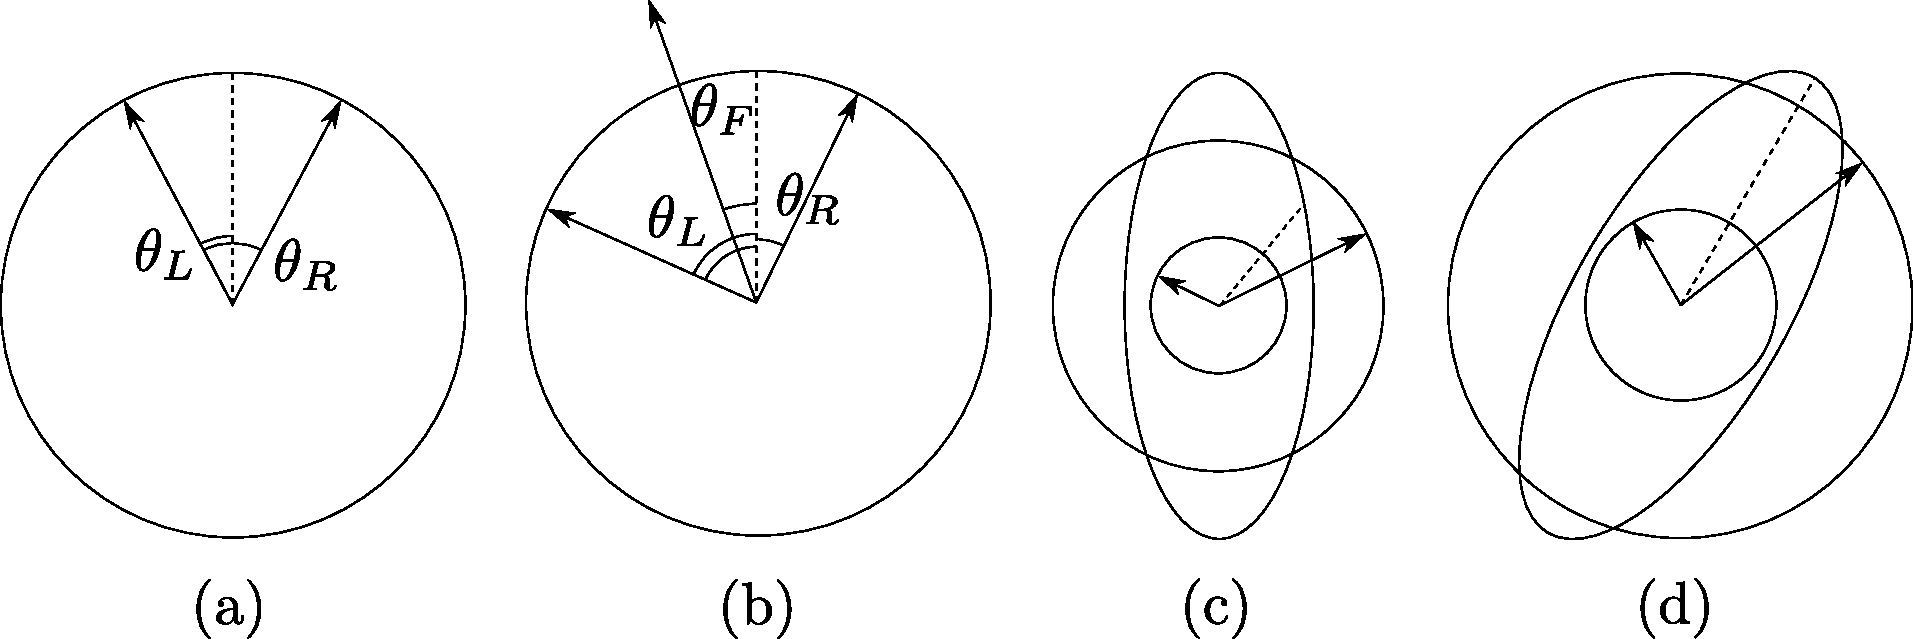
\includegraphics[scale=0.4]{faraday.pdf}
  \caption{}
  \label{faraday}
\end{figure}

物質中を$l$進んだ後の直線偏光の旋回角$\theta_F$は,
\begin{align}
  \theta_F &=  - \dfrac{\theta_R - \theta_L}{2}\notag \\
  &= \dfrac{2\pi(n_ -  - n_+)l}{2\lambda}\notag \\
  &=  - \pi\Delta{n}\dfrac{l}{\lambda} \label{faraday_eff_thetaF}
\end{align}
また,楕円偏光の楕円率(長軸と短軸の比)$\eta_F$は,
\begin{align}
  \eta_F &= \dfrac{E_L - E_R}{E_L+E_R}\notag \\
  &= \dfrac{\exp\left( - \dfrac{\kappa_+\omega{l}}{c}\right) - \exp\left( - \dfrac{\kappa_ - \omega{l}}{c}\right)}{\exp\left( - \dfrac{\kappa_+\omega{l}}{c}\right)+\exp\left( - \dfrac{\kappa_ - \omega{l}}{c}\right)}\notag \\
  &\sim  - \pi\Delta{\kappa}\dfrac{l}{\lambda} \label{faraday_eff_etaF}
\end{align}
となる.よって,\eqref{faraday_eff_deltan},\eqref{faraday_eff_deltakappa},\eqref{faraday_eff_thetaF},\eqref{faraday_eff_etaF}から,
\begin{align}
  \theta_F &=  - \dfrac{\omega}{2c}\cdot\dfrac{\kappa\varepsilon'_{\xi\eta} - n\varepsilon''_{\xi\eta}}{n^2+\kappa^2}l \\
  \eta_F &=  - \dfrac{\omega}{2c}\cdot\dfrac{n\varepsilon'_{\xi\eta}+\kappa\varepsilon''_{\xi\eta}}{n^2+\kappa^2}l
\end{align}
となる.
これは等方性媒質に対し,外部から磁場をかけて異方的にした効果である.

\paragraph{複素電磁波動方程式}
Faraday効果で複素屈折率という概念を導入した.振動子モデルでは複素感受率や複素誘電率である誘電関数も出てきた.
実数の物理量であった$n$,$\varepsilon$には,
\begin{align}
  \frac{c}{n}=\sqrt{\varepsilon\mu_0}
\end{align}
が成立し,さらに,電場に対しては波動方程式
\begin{align}
  \nabla^2\boldsymbol{E}=\varepsilon\mu_0\dfrac{\partial^2\boldsymbol{E}}{\partial{t}^2}
\end{align}
が成立した.

Faraday効果の項目で導入した複素物理量について復習しておく.
物質の中を電磁波が伝播するときは,一般にそのエネルギーは散逸し,振幅は減衰する.その度合いを消失係数$\kappa$で表す.
また,\textbf{物質中を伝わる電磁波の減衰は距離の指数関数で表される}.
これをLambert-Beerの法則という.よって,物質中で$x$だけ進んで,振幅が$A$倍になったときに
\begin{align}
  A=\exp\left(-\dfrac{\kappa\omega{x}}{c}\right)
\end{align}
で消失係数$\kappa$を定義する.屈折率$n$の物質中で電磁波が$x$伝わった時の電場は,
\begin{align}
  \boldsymbol{E}=\boldsymbol{E}_0\exp\left(-\dfrac{\kappa\omega{x}}{c}\right)\exp\left[-i\omega\left(t-\dfrac{x}{c/n}\right)\right] = \boldsymbol{E}_0\exp\left[-i\omega{t}+i\dfrac{\omega{x}}{c/N}\right]\label{comp_wave_eq_E}
\end{align}
で表される.$x=0$での振幅を$\boldsymbol{E}_0$とする.ここで,複素屈折率$N$
\begin{align}
  N=n+i\kappa
\end{align}
を導入した.
この$N$によって,位相変化の項の中に減衰も含めることができるのだ.
さらに,複素波数$K$を
\begin{align}
  \boldsymbol{K}=N\boldsymbol{k}=(n+i\kappa)\boldsymbol{k}
\end{align}
で定義する.この複素波数を用いると,(\ref{comp_wave_eq_E})は,
\begin{align}
  \boldsymbol{E}=\boldsymbol{E}_0\exp\left[i\left(\boldsymbol{K}\cdot\boldsymbol{r}-\omega{}t\right)\right]\label{comp_wave_eq_Ek}
\end{align}
と書くことができる.さらに,複素屈折率ベクトル$\boldsymbol{N}$を
\begin{align}
  \boldsymbol{N}=\dfrac{N}{k}\boldsymbol{k}\label{comp_wave_eq_def_N}
\end{align}
で定義すると,
\begin{align}
  \boldsymbol{E}=\boldsymbol{E}_0\exp\left[i\left(\dfrac{\omega}{c}\boldsymbol{N}\cdot\boldsymbol{r}-\omega{}t\right)\right]\label{comp_wave_eq_Eomega}
\end{align}
と書くこともできる.結局,
(\ref{comp_wave_eq_Ek}),(\ref{comp_wave_eq_Eomega})において,
\begin{quote}
  複素波数$\boldsymbol{K}$もしくは複素屈折率$N$の虚部が正だと減衰が起こる
\end{quote}
と言える.

複素数に対応する波動方程式は\eqref{comp_wave_eq_def_N}\eqref{comp_wave_eq_Eomega}から
\begin{align}
  \nabla^2 \boldsymbol{E} &= \left(\dfrac{i\omega{N}}{c}\right)^2 \boldsymbol{E}\\
  \dfrac{\partial^2\boldsymbol{E}}{\partial{t}^2} &= (i\omega)^2 \boldsymbol{E}
\end{align}
となる.これらから,減衰を複素屈折率として取り入れた電磁波動方程式
\begin{align}
  \nabla^2 \boldsymbol{E} = \left(\dfrac{1}{c/N}\right)^2\dfrac{\partial^2\boldsymbol{E}}{\partial{t}^2}\label{comp_wave_eq_comp_wave}
\end{align}
が導かれる.
振動子モデルで扱った散逸を無視しない誘電関数の形は,
\begin{align}
  \varepsilon(\omega)=\varepsilon_0\left(\dfrac{\varepsilon_{\text{b}}}{\varepsilon_0}+\dfrac{{\omega_p}^2}{{\omega_0}^2-\omega^2-i\gamma\omega}\right)\label{comp_wave_eq_permittivity}
\end{align}
となる.電荷分布や電流分布がないMaxwell方程式は,
\begin{align}
  \dive{\boldsymbol{E}}&=0\label{comp_wave_eq_dive}\\
  \text{rot}{\boldsymbol{E}}&=-\dfrac{\partial\boldsymbol{B}}{\partial{t}}\label{comp_wave_eq_rote}\\
  \text{rot}{\boldsymbol{B}}&=\varepsilon(\omega)\mu_0\dfrac{\partial\boldsymbol{E}}{\partial{t}}\label{comp_wave_eq_rotb}\\
  \dive{\boldsymbol{B}}&=0\label{comp_wave_eq_divb}
\end{align}
となる.(\ref{comp_wave_eq_dive}),(\ref{comp_wave_eq_rote}),(\ref{comp_wave_eq_rotb})から,
\begin{align}
  \nabla^2\boldsymbol{E}=\varepsilon(\omega)\mu_0\dfrac{\partial^2\boldsymbol{E}}{\partial{t}^2}
\end{align}
となる.これと(\ref{comp_wave_eq_comp_wave}),(\ref{comp_wave_eq_permittivity})から,
\begin{align}
  N &= n+i\kappa\notag\\
  &=\sqrt{1+\dfrac{{\omega_p}^2}{{\omega_0}^2-\omega^2-i\gamma\omega}}
\end{align}
となることが分かる.結局,複素数に拡張した電磁波動方程式は,
\begin{align}
  \nabla^2\boldsymbol{E} &= \left(\dfrac{\varepsilon_{\text{b}}}{\varepsilon_0}+\dfrac{{\omega_p}^2}{{\omega_0}^2-\omega^2-i\gamma\omega}\right)\varepsilon_0\mu_0\dfrac{\partial^2\boldsymbol{E}}{\partial{t}^2}\notag\\
  &= \left[n(\omega)^2-\kappa(\omega)^2+2in(\omega)\kappa(\omega)\right]\varepsilon_0\mu_0\dfrac{\partial^2\boldsymbol{E}}{\partial{t}^2}\label{comp_wave_eq_newequationE}
\end{align}
と書き直される.(\ref{comp_wave_eq_newequationE})は分散と減衰も考慮した式である.磁束密度に関する方程式も,
\begin{align}
  \nabla^2\boldsymbol{B} &= \left(\dfrac{\varepsilon_{\text{b}}}{\varepsilon_0}+\dfrac{{\omega_p}^2}{{\omega_0}^2-\omega^2-i\gamma\omega}\right)\varepsilon_0\mu_0\dfrac{\partial^2\boldsymbol{B}}{\partial{t}^2}\notag\\
  &= \left[n(\omega)^2-\kappa(\omega)^2+2in(\omega)\kappa(\omega)\right]\varepsilon_0\mu_0\dfrac{\partial^2\boldsymbol{B}}{\partial{t}^2}\label{comp_wave_eq_newequationB}
\end{align}
のように同じ形で表される.
ここで,必ずしも散逸$\gamma$が存在しない(誘電率が実数である)からと言って,消衰$\kappa$が存在しないという訳ではないことに注意.

\paragraph{異方性媒質}
異方性のある媒質中で任意の方向へ進む光について考える.

異方性媒質の誘電率テンソルは一般に,
\begin{align}
  \begin{pmatrix}
    \varepsilon_{11} & \varepsilon_{12} & \varepsilon_{13}\\
    \varepsilon_{21} & \varepsilon_{22} & \varepsilon_{21}\\
    \varepsilon_{31} & \varepsilon_{32} & \varepsilon_{33}
  \end{pmatrix}
\end{align}
と書くことができる.ここで,物質に対し適当な座標系を選ぶと,誘電率テンソルの対角成分以外を0にすることが可能な場合がある.
この場合の座標軸をテンソルの主軸と言い,対角成分を主値と言う.ここで,主軸と主値は物体固有のものである.

主値のうち,2つが一致している時を1軸性の異方性と言い,異なる主値を持つ成分の軸を光学軸と言う.主値がどれも一致していない時は2軸性の異方性と呼ぶ.
以下では媒質が透明で,透磁率が等方的で$\mu$の場合を考える.

Maxwell方程式から,平面波について
\begin{align}
  \rot\boldsymbol{E}&=\boldsymbol{k}\times\boldsymbol{E}=\omega\mu\boldsymbol{H}\label{aniso_kE}\\
  \rot\boldsymbol{H}&=\boldsymbol{k}\times\boldsymbol{H}=-\omega\boldsymbol{D}=-\omega\varepsilon\boldsymbol{E}\label{aniso_kH}
\end{align}
となる.
Poyntingベクトル$\boldsymbol{S}$は\eqref{aniso_kE}\eqref{aniso_kH}から,
\begin{align}
  \boldsymbol{S}=\boldsymbol{E}\times\boldsymbol{H}=\dfrac{1}{\mu\omega}\left[E^2\boldsymbol{k}-(\boldsymbol{k}\cdot\boldsymbol{E})\boldsymbol{E}\right]
\end{align}
で表される.このように,異方性媒質中では波の伝播方向とエネルギーの流れる方向が異なっている.
以上から,$\boldsymbol{k}$, $\boldsymbol{E}$, $\boldsymbol{D}$, $\boldsymbol{H}$, $\boldsymbol{S}$の関係は図のようになる.
$\boldsymbol{k}$, $\boldsymbol{E}$, $\boldsymbol{D}$, $\boldsymbol{S}$は同一平面内に存在する.
さらに,$\boldsymbol{H}$はこの平面に直交する.

\begin{figure}[ht]
  \centering
  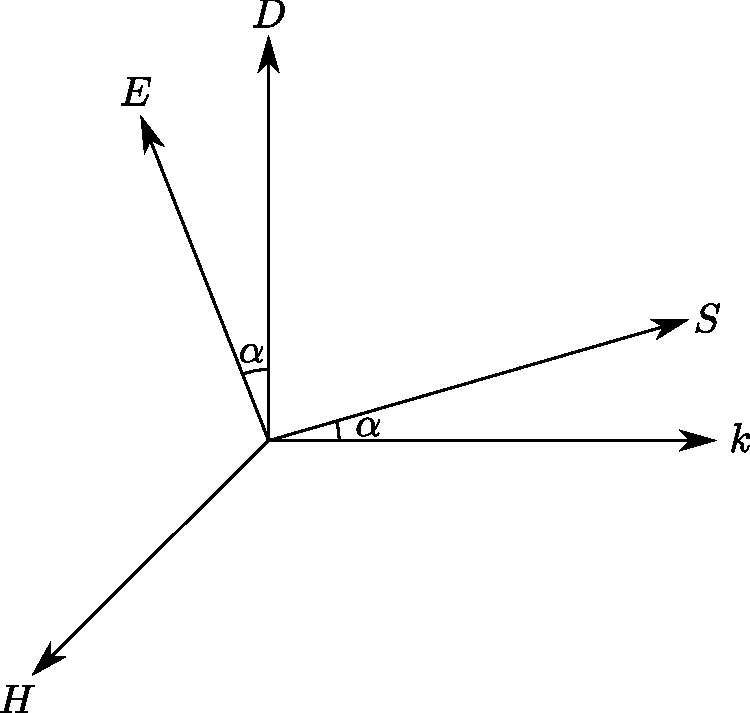
\includegraphics[scale=0.5]{vectors.pdf}
  \caption{主要なベクトルの関係図}
  \label{vectors}
\end{figure}

ここで,
\begin{align}
  \boldsymbol{n}=\dfrac{c}{\omega}\boldsymbol{k}\label{aniso_nvec}
\end{align}
で屈折率ベクトル$\boldsymbol{n}$を定義する.$c$は真空中の光速である.ただし,屈折率ベクトルの絶対値はその向きによって変わる.
また,\eqref{aniso_kE}\eqref{aniso_kH}から,
\begin{align}
  \sum_j(n^2\delta_{ij}-n_i{}n_j-\mu{}c^2\varepsilon_{ij})E_j=0\label{aniso_fresE}
\end{align}
となる.ただし,$\delta_{ij}$はクロネッカーのデルタである.これが$\boldsymbol{E}=0$以外の解を持つには,
\begin{align}
  \text{det}(n^2\delta_{ij}-n_i{}n_j-\mu{}c^2\varepsilon_{ij})=0
\end{align}
であればよい.これを計算するときはテンソルの主軸となる座標系へ移行すると楽である.これを展開すると,6次の項はなくなり,
\begin{align}
  n^2(\varepsilon_{\xi}{n_\xi}^2+\varepsilon_{\eta}{n_\eta}^2+\varepsilon_{\zeta}{n_\zeta}^2)
  -\mu{c}^2\left[{n_\xi}^2\varepsilon_\xi(\varepsilon_\eta+\varepsilon_\zeta)
  +{n_\eta}^2\varepsilon_\eta(\varepsilon_\zeta+\varepsilon_\xi)
  +{n_\zeta}^2\varepsilon_\zeta(\varepsilon_\eta+\varepsilon_\xi)\right] \notag \\
  +\mu^2{c}^4\varepsilon_\xi\varepsilon_\eta\varepsilon_\zeta = 0 . \label{aniso_fresEq}
\end{align}
ただし,テンソルの主値$\varepsilon_{ii}$を$\varepsilon_{i}$とした.これをFresnel方程式と呼ぶ.
Fresnel方程式\eqref{aniso_fresEq}は$n_\xi$, $n_\eta$, $n_\zeta$座標で4次曲面をなす.これを屈折率ベクトル面と呼ぶ.
屈折率ベクトル面は\eqref{aniso_fresEq}から分かるように$\omega$にも依存している.
そして,$\boldsymbol{n}$の方向が決まっている時は\eqref{aniso_fresEq}は$n$に関する2次方程式となるので,一般に2つの解を持つ.
つまり,$\boldsymbol{n}$の方向が決まっている時はその絶対値は2つ存在するということが分かる.

さらに,等方性媒質の中では群速度$\boldsymbol{v}_s$と波数$\boldsymbol{k}$の向きは一致しているが,異方性媒質では一致していない.
異方性媒質中では群速度が光線の方向と一致している.そこで,向きが群速度の向きと一致しており,大きさが
\begin{align}
  \boldsymbol{s}\cdot\boldsymbol{n}=1 \label{aniso_def_s}
\end{align}
となる光線ベクトル$\boldsymbol{s}$を定義する.

\eqref{aniso_kE}\eqref{aniso_kH}\eqref{aniso_nvec}から,
\begin{align}
  \boldsymbol{n}\times\boldsymbol{E} &= \mu{c}\boldsymbol{H}\label{aniso_nE}\\
  \boldsymbol{n}\times\boldsymbol{H} &= -c\boldsymbol{D}\label{aniso_nH}
\end{align}
となる.\eqref{aniso_nE}\eqref{aniso_nH}と定義$\boldsymbol{s}\cdot\boldsymbol{n}=1$から,
\begin{align}
  \boldsymbol{s}\times\boldsymbol{D} &= \boldsymbol{s}\times\left[-\dfrac{1}{c}\boldsymbol{n}\times\boldsymbol{H}\right]\notag\\
  &= -\dfrac{1}{c}\left[(\boldsymbol{s}\cdot\boldsymbol{H})\boldsymbol{n}-(\boldsymbol{s}\cdot\boldsymbol{n})\boldsymbol{H}\right]\notag\\
  &= \dfrac{\boldsymbol{H}}{c} . \label{aniso_sxD}
\end{align}
同様に,
\begin{align}
  \boldsymbol{s}\times\boldsymbol{H}=-\dfrac{1}{\mu{}c}\boldsymbol{E}\label{aniso_sxH}
\end{align}
となる.
\eqref{aniso_sxD}\eqref{aniso_sxH}から,Fresnel方程式を導いたのと同様の議論から,
\begin{align*}
  \text{det}\left(\delta_{ij}s^2\varepsilon_{ij}-\dfrac{\delta_{ij}}{\mu{}c^2}-s_is_j\varepsilon_{ij}\right)=0
\end{align*}
となり,これを展開すると,
\begin{align}
  s^2(\varepsilon_\eta\varepsilon_\zeta{s_\xi}^2+\varepsilon_\zeta\varepsilon_\xi{s_\eta}^2+\varepsilon_\xi\varepsilon_\eta{s_\zeta}^2)
  -\dfrac{1}{\mu{}c^2}\left[{s_\xi}^2(\varepsilon_\eta+\varepsilon_\zeta)+{s_\eta}^2(\varepsilon_\zeta+\varepsilon_\xi)+{s_\zeta}^2(\varepsilon_\xi+\varepsilon_\eta)\right]
  +\dfrac{1}{\mu^2c^4}=0
\end{align}
となる.これを光線速度面方程式と呼ぶ.ただし,主値の添字は略した.これは$(s_\xi,s_\eta,s_\zeta)$座標において4次曲面をなす.これを光線速度面と呼ぶ.

さて,波動光学の近似として幾何光学が有効なのは,問題にしているスケールが波長$\lambda$より十分大きい時だけ.
この条件の下,位置や時間による誘電率の変化は緩やかで,位相は屈折率を光の進路にそって積分した光路長によって表すことができるとする近似をアイコナール近似と呼ぶ.
アイコナール近似では,電場や磁場が
\[\psi(\boldsymbol{r})=a(\boldsymbol{r})\exp[i(k\phi(\boldsymbol{r})-\omega{}t)]\]
と表される時,この$\phi(\boldsymbol{r})$をアイコナールと呼ぶ.
定義と\eqref{aniso_nvec}から,
\begin{align}
  \grad\phi(\boldsymbol{r}) = \boldsymbol{n}.\label{aniso_gradphi}
\end{align}

次に等位相面について考える.アイコナールを含んだ位相は$k\phi-\omega{t}$であるので,ある時刻$t_0$において,
\begin{align}
  \phi = \phi_0 = \text{const}.
\end{align}
で決定される曲面が等位相面である.さらに,微小時間$\delta{t}$経過した後,この等位相面は,
\begin{align}
  k\phi_0-\omega{t_0}=k(\phi_0+\delta\phi)-\omega(t_0+\delta{t})\label{aniso_phidev}
\end{align}
で与えられる$\delta\phi$を用いて,
\begin{align}
  \phi=\phi_0+\delta\phi.
\end{align}
また,\eqref{aniso_phidev}から,
\begin{align}
  \delta\phi=\dfrac{\omega}{k}\delta{t}.
\end{align}
一般に,曲面$\phi(\xi,\eta,\zeta)=\phi_0$上の1点P$_0(\xi_0,\eta_0,\zeta_0)$の近くにP$(\xi_0+\delta\xi,\eta_0+\delta\eta,\zeta_0+\delta\zeta)$を取る.
P$_0$及びPは共に等位相面上にあるので,
\[\phi(\xi_0,\eta_0,\zeta_0)=\phi(\xi_0+\delta\xi,\eta_0+\delta\eta,\zeta_0+\delta\zeta)=\phi_0.\]
最左辺を展開して1次まで取ると,中辺と合わせて,
\[\dfrac{\partial\phi}{\partial\xi}\delta\xi+\dfrac{\partial\phi}{\partial\eta}\delta\eta+\dfrac{\partial\phi}{\partial\zeta}\delta\zeta=0.\]
よって,等位相面内の任意の微小ベクトルを$\delta{\boldsymbol{r}}=(\delta\xi,\delta\eta,\delta\zeta)$を用いると,\eqref{aniso_gradphi}と合わせて,
\begin{align}
  \text{grad}\,\phi(\boldsymbol{r})\cdot\delta\boldsymbol{r}=\boldsymbol{n}\cdot\delta\boldsymbol{r}=0.\label{aniso_ndr}
\end{align}
よって,$(\xi,\eta,\zeta)$座標において屈折率ベクトル$\boldsymbol{n}$は等位相面に対し直交する事が分かる.

% <!--
%
% Fermatの原理から,空間内のある点Aから別の点Bへ進む光の経路は,その経路に沿っての線積分
% \begin{align}
%   \phi=\int_{\text A}^{\text B}\boldsymbol{n}\cdot{}d\boldsymbol{l}=\int_{\text A}^{\text B}ndl
% \end{align}
% が極小になるという条件で決定される.ところで,では群速度$\boldsymbol{v}_s$と光線の向き$l$は平行なので,
% \begin{align}
%   \phi=\int\boldsymbol{n}\cdot{}d\boldsymbol{l}=\int\boldsymbol{n}\cdot\left(\dfrac{\boldsymbol{s}}{s}dl\right)=\int\dfrac{dl}{s}
% \end{align}
% となる.均質な媒質中では$s$は光線に沿って一定であるので,考えている光の経路の長さを$L$とすると,$\phi=\dfrac{L}{s}$となる.これから明らかなように,
% 光束の中心から出る各動径方向で$s$に等しい線分の端点が作る曲面は等位相面となる.これを光線速度面と呼ぶ.
%
% -->

\eqref{aniso_fresEq}のFresnel方程式は$n_i$を使って記述されているが,屈折率ベクトル面を$f(k_\xi,k_\eta,k_\zeta,\omega)=0$で記述することにすると,偏微分の一般的な公式\footnote{\(f=f(k, \omega)\)を変形して\(\omega=\Omega(f, k)\)とする.\(\omega = \Omega(f(k, \omega), k)\)となる.両辺を\(k\)で偏微分すれば\(0 = (\partial\Omega/\partial f)(\partial f/\partial k) + (\partial\Omega/\partial k)\)}から
\[
(v_s)_i = \left( \dfrac{\partial\omega}{\partial{}k_i} \right)_f
= -\dfrac{\left(\cfrac{\partial{f}}{\partial{}k_i}\right)_\omega}{\left(\cfrac{\partial{}f}{\partial\omega}\right)_{k_i}}
= -\dfrac{c}{\omega}\dfrac{\left(\cfrac{\partial{f}}{\partial{}n_i}\right)_\omega}{\left(\cfrac{\partial{}f}{\partial\omega}\right)_{k_i}}
\]
となる.最後の式に移るときは,$\omega$一定という条件で偏微分していることを利用した.
ところで,$\dfrac{\partial{f}}{\partial\boldsymbol{n}}$は曲面$f=0$の法線方向を向いている.
よって,光線ベクトル$\boldsymbol{s}$は屈折率ベクトル面の対応する点における法線の向きを向いていることが分かる.
屈折率ベクトル面は$(n_\xi,n_\eta,n_\zeta)$座標において定義されていることに注意.これは
\begin{align}
  \boldsymbol{s}\cdot\delta\boldsymbol{n}=0\label{aniso_sdn}
\end{align}
と表される.さらに,$\boldsymbol{s}$の定義$\boldsymbol{s}\cdot\boldsymbol{n}=1$を$\omega=\text{const}$の下で両辺微分して,
$\boldsymbol{s}\cdot\delta\boldsymbol{n}+\boldsymbol{n}\cdot\delta\boldsymbol{s}=0$となるので,\eqref{aniso_sdn}から,
\begin{align}
  \boldsymbol{n}\cdot\delta\boldsymbol{s}=0.\label{aniso_nds}
\end{align}
\eqref{aniso_ndr}\eqref{aniso_nds}から,$\delta\boldsymbol{r}$が等位相面内の任意の微小ベクトルであることを考慮すると,$(\xi,\eta,\zeta)$座標において原点から伸ばした光線ベクトル$\boldsymbol{s}$が作る面は等位相面である.
また,\eqref{aniso_nds}から,屈折率ベクトル$\boldsymbol{n}$は光線速度面の対応する点における法線の向きを向いていることが分かる.
光線速度面は$(s_\xi,s_\eta,s_\zeta)$座標において定義されていることに注意.
屈折率ベクトル$\boldsymbol{n}$と同様に,ある1点を出た光であっても,$\boldsymbol{s}$はその向きによって絶対値が変わる.

ここで,Poyntingベクトル$\boldsymbol{S}$と光線ベクトル$\boldsymbol{s}$の関係を求める.\eqref{aniso_kE}と\eqref{aniso_kH}を微分して,
\begin{align*}
  \delta\boldsymbol{D} &= -\dfrac{1}{\omega}[\delta\boldsymbol{k}\times\boldsymbol{H}+\boldsymbol{k}\times\delta\boldsymbol{H}] , \\
  \delta\boldsymbol{H} &= \dfrac{1}{\omega\mu}[\delta\boldsymbol{k}\times\boldsymbol{E}+\boldsymbol{k}\times\delta\boldsymbol{E}] .
\end{align*}
それぞれの両辺で$\boldsymbol{E}$, $\boldsymbol{H}$とのスカラー積を取ると,
\begin{align*}
  \boldsymbol{E}\cdot\delta\boldsymbol{D} = -\dfrac{1}{\omega}[\boldsymbol{E}\cdot(\delta\boldsymbol{k}\times\boldsymbol{H})+\boldsymbol{E}\cdot(\boldsymbol{k}\times\delta\boldsymbol{H})] , \\
  \mu\boldsymbol{H}\cdot\delta\boldsymbol{H} = \dfrac{1}{\omega}[\boldsymbol{H}\cdot(\delta\boldsymbol{k}\times\boldsymbol{E})+\boldsymbol{H}\cdot(\boldsymbol{k}\times\delta\boldsymbol{E})] .
\end{align*}
ここで,ベクトル解析の公式
\[a\cdot(b\times{}c)=(a\times{}b)\cdot{}c\]
及び$\varepsilon_{ij}$の対称性から導かれる式
\[\boldsymbol{D}\cdot\delta\boldsymbol{E}=\sum_i\sum_j\varepsilon_{ij}E_j\delta{}E_i=\sum_i\sum_jE_j\varepsilon_{ji}\delta{}E_i=\boldsymbol{E}\cdot\delta\boldsymbol{D}\]
と\eqref{aniso_kE}と\eqref{aniso_kH}を使うと,
\begin{align*}
  \boldsymbol{E}\cdot\delta\boldsymbol{D} = \dfrac{1}{\omega}(\boldsymbol{E}\times\boldsymbol{H})\cdot\delta\boldsymbol{k}+\mu\boldsymbol{H}\cdot\delta\boldsymbol{H}\\
  \mu\boldsymbol{H}\cdot\delta\boldsymbol{H} = \dfrac{1}{\omega}(\boldsymbol{E}\times\boldsymbol{H})\cdot\delta\boldsymbol{k}+ \boldsymbol{E}\cdot\delta\boldsymbol{D}
\end{align*}
となる.この2式から,$\boldsymbol{k}\parallel\boldsymbol{n}$を考慮すると,
\begin{align}
  (\boldsymbol{E}\times\boldsymbol{H})\cdot\delta\boldsymbol{n}=\boldsymbol{S}\cdot\delta\boldsymbol{n}=0\label{aniso_Sdn}
\end{align}
となる.\eqref{aniso_sdn}\eqref{aniso_Sdn}から,群速度もしくは光線ベクトルとPoyntingベクトルは同じ向きを向いていることが分かる.よって,
\begin{align}
  \boldsymbol{s}\cdot\boldsymbol{H} &= 0\label{aniso_sE}\\
  \boldsymbol{s}\cdot\boldsymbol{E} &= 0.\label{aniso_sH}
\end{align}

異方性媒質中を伝播する光の偏りについて考える.
Fresnel方程式\eqref{aniso_fresEq}を導くきっかけとなった方程式\eqref{aniso_fresE}には電場$\boldsymbol{E}$が含まれている.
だが,$\boldsymbol{k}$と$\boldsymbol{E}$は異なる方向を向いているので,光波の偏りを考えるのには適していない.
図を見ると,$\boldsymbol{k}$と電束密度$\boldsymbol{D}$が直交している.
なので,電束密度$\boldsymbol{D}$を基に式を立て直す.\eqref{aniso_nE}\eqref{aniso_nH}から,
\begin{align}
  \boldsymbol{D}=\dfrac{1}{\mu{c}^2}\left[n^2\boldsymbol{E}-(\boldsymbol{n}\cdot\boldsymbol{E})\boldsymbol{n}\right].\label{aniso_newD}
\end{align}
ここで,新しい式を立てる際に,座標軸が屈折率ベクトル$\boldsymbol{n}$もしくは波数$\boldsymbol{k}$の方を向くようにする.
さらに,この座標系の残りの軸を1,2軸とし,$\alpha=1,2$, $\beta=1,2$とする.$\alpha$軸は$\boldsymbol{n}$と直交するので,\eqref{aniso_newD}の$\alpha$成分は
\[D_\alpha=\dfrac{n^2}{\mu{}c^2}E_\alpha\]
となる.さらに,誘電率の2階逆テンソル$\varepsilon_{\alpha\beta}^{-1}$を考え,
\[E_\alpha=\sum_{\beta}\varepsilon_{\alpha\beta}^{-1}D_\beta.\]
これら2式から,
\begin{align}
  D_\alpha-\dfrac{n^2}{\mu{}c^2}\sum_\beta\varepsilon_{\alpha\beta}^{-1}D_\beta=0
\end{align}
もしくは
\begin{align}
  \left(\dfrac{\mu{}c^2}{n^2}\delta_{\alpha\beta}-\varepsilon_{\alpha\beta}^{-1}\right)D_\beta=0
\end{align}
となる.これはテンソルの固有値問題となっていて,あらわに書けば,
\begin{align}
  \begin{pmatrix}
    \varepsilon^{-1}_{11}-\left(\dfrac{\mu{c^2}}{n^2}\right) & \varepsilon^{-1}_{12}\\
    \varepsilon^{-1}_{21} & \varepsilon^{-1}_{22}-\left(\dfrac{\mu{c^2}}{n^2}\right)
  \end{pmatrix}
  \begin{pmatrix}
    D_1\\
    D_2
  \end{pmatrix}
  =0\label{aniso_newDeq}
\end{align}
が得られる.$\boldsymbol{D}$などのベクトルと誘電率テンソル$\varepsilon$は座標系によって異なる成分を返すことに注意.

\eqref{aniso_newDeq}が$D_1=D_2=0$以外の解を持つ条件は,行列式が0となることなので,
\begin{align}
  \dfrac{\mu{}c^2}{n^2}=\dfrac{\varepsilon^{-1}_{11}+\varepsilon^{-1}_{22}\pm\sqrt{(\varepsilon^{-1}_{11}-\varepsilon^{-1}_{22})^2+4\varepsilon^{-1}_{12}\varepsilon^{-1}_{21}}}{2}
\end{align}
となる.また,先程も述べたように,$\boldsymbol{n}$の向きが決まっている時,その絶対値$n$は2つ存在する.
この式から,確かに$n$は2つ存在することが分かる.それを$n^{(1)}$, $n^{(2)}$とする.
\eqref{aniso_newDeq}の行列式が0になるという条件はもとの$(\xi,\eta,\zeta)$座標におけるFresnel方程式に一致する.
この座標系は$\varepsilon$の主軸であった.さて,\eqref{aniso_newDeq}を見ると,$n^{(1)}$と$n^{(2)}$に対応する二つの$\boldsymbol{D^{(1)}}$と$\boldsymbol{D^{(2)}}$が存在し,それらは$\varepsilon^{-1}$の固有ベクトル(主軸)である.
一般に,固有ベクトル同士は直交するので,$\boldsymbol{D^{(1)}}$と$\boldsymbol{D^{(2)}}$は$(1,2)$平面内で直交する.
先ほどの固有値問題は2次元テンソルについて考えていたことに注意.
ところが,双方とも$\boldsymbol{n}$に直交する平面つまり$(1,2)$平面内にのみ存在することは分かっているので,結局,
\begin{align}
  \boldsymbol{D^{(1)}}\cdot\boldsymbol{D^{(2)}}=0
\end{align}
となる.同じ向きの屈折率ベクトルを持つ2つの光波の電束密度は互いに直交することが分かった.

\eqref{aniso_newDeq}を幾何的に表す.誘電率テンソルの主軸である$(\xi,\eta,\zeta)$座標における$\varepsilon^{-1}$に対応するテンソル楕円体
\begin{align}
  \sum_i\sum_k\varepsilon^{-1}_{ik}r_ir_k=\mu{c^2}=\dfrac{1}{\varepsilon_0}\label{aniso_tensEll}
\end{align}
を考える.$r_1,r_2,r_3$はそれぞれ$\xi,\eta,\zeta$を示す.$\varepsilon$の主軸は$\varepsilon^{-1}$の主軸にもなるので,$(\xi,\eta,\zeta)$においては
\begin{align}
  \varepsilon^{-1}
  =
  \begin{pmatrix}
    \dfrac{1}{\varepsilon_\xi} & 0 & 0 \\
    0 & \dfrac{1}{\varepsilon_\eta} & 0 \\
    0 & 0 & \dfrac{1}{\varepsilon_\zeta}
  \end{pmatrix}\label{aniso_inverse}
\end{align}
の形で表される.\eqref{aniso_tensEll}を\eqref{aniso_inverse}に代入して,
\begin{align}
  \dfrac{\xi^2}{\varepsilon_\xi/\varepsilon_0}+\dfrac{\eta^2}{\varepsilon_\eta/\varepsilon_0}+\dfrac{\zeta^2}{\varepsilon_\zeta/\varepsilon_0}=1\label{aniso_nEll}
\end{align}
となる.これを屈折率楕円体と呼ぶ.

\begin{figure}[ht]
  \centering
  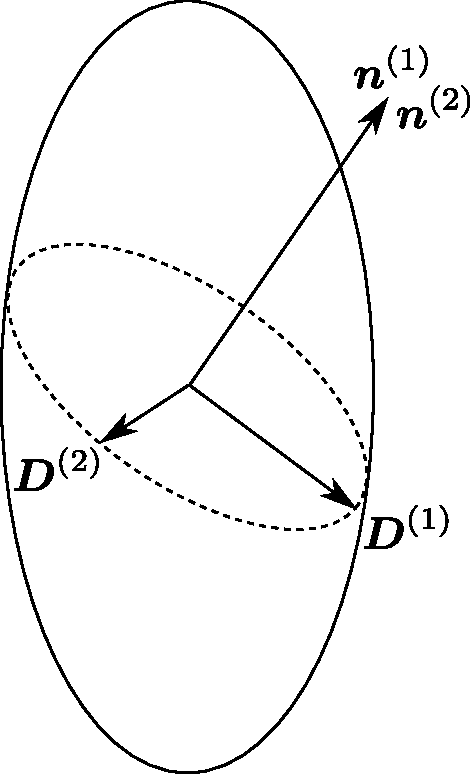
\includegraphics[scale=0.4]{nEllipse.pdf}
  \caption{屈折率楕円体}
  \label{nEllipse}
\end{figure}

屈折率楕円体の$\xi$軸,$\eta$軸,$\zeta$軸との交点の値$\sqrt{\dfrac{\varepsilon_\xi}{\varepsilon_0}}$, $\sqrt{\dfrac{\varepsilon_\eta}{\varepsilon_0}}$, $\sqrt{\dfrac{\varepsilon_\zeta}{\varepsilon_0}}$を主屈折率と呼ぶ.

中心を通り,$\boldsymbol{n}$に垂直な面で屈折率楕円体を切る.この平面の式は,
\begin{align}
  n_\xi\xi+n_\eta\eta+n_\zeta\zeta=0\label{aniso_plane}
\end{align}
で与えられる.切断面の楕円の長軸と短軸を求める.これは,\eqref{aniso_nEll}\eqref{aniso_plane}のもとで
\begin{align}
  r^2=\xi^2+\eta^2+\zeta^2
\end{align}
の極値を求めることに等しい.これにはLagrangeの未定乗数法を使う.
\begin{align}
  F=\xi^2+\eta^2+\zeta^2+2\lambda_1\left(n_\xi\xi+n_\eta\eta+n_\zeta\zeta\right)+\lambda_2\left(\dfrac{\xi^2}{\varepsilon_\xi/\varepsilon_0}+\dfrac{\eta^2}{\varepsilon_\eta/\varepsilon_0}+\dfrac{\zeta^2}{\varepsilon_\zeta/\varepsilon_0}-1\right)
\end{align}
となる$F$に対し,
\begin{align*}
  \dfrac{\partial{F}}{\partial\xi}=2\xi+2\lambda_1n_\xi+2\lambda_2\dfrac{\xi}{\varepsilon_\xi/\varepsilon_0}=0\\
  \dfrac{\partial{F}}{\partial\eta}=2\eta+2\lambda_1n_\eta+2\lambda_2\dfrac{\eta}{\varepsilon_\eta/\varepsilon_0}=0\\
  \dfrac{\partial{F}}{\partial\zeta}=2\zeta+2\lambda_1n_\zeta+2\lambda_2\dfrac{\zeta}{\varepsilon_\zeta/\varepsilon_0}=0
\end{align*}
を解けばよい.これらから,
\begin{align}
  \begin{split}
    \left(1+\dfrac{\lambda_2}{\varepsilon_\xi/\varepsilon_0}\right)\xi+\lambda_1n_\xi=0\\
    \left(1+\dfrac{\lambda_2}{\varepsilon_\eta/\varepsilon_0}\right)\eta+\lambda_1n_\eta=0\\
    \left(1+\dfrac{\lambda_2}{\varepsilon_\zeta/\varepsilon_0}\right)\zeta+\lambda_1n_\zeta=0
  \end{split}
  \label{aniso_lag1}
\end{align}
両辺に$\xi,\eta,\zeta$をかけて足し合わせると,
\begin{align}
  \xi^2+\eta^2+\zeta^2+\lambda_2\left(\dfrac{\xi^2}{\varepsilon_\xi/\varepsilon_0}+\dfrac{\eta^2}{\varepsilon_\eta/\varepsilon_0}+\dfrac{\zeta^2}{\varepsilon_\zeta/\varepsilon_0}\right)+\lambda_1\left(n_\xi\xi+n_\eta\eta+n_\zeta\zeta\right) .
\end{align}
\eqref{aniso_nEll}\eqref{aniso_plane}より,第2項は1,第3項は0となるので,
\begin{align}
  r^2+\lambda_2=0 . \label{aniso_lambda2}
\end{align}
\eqref{aniso_lag1}両辺に$n_\xi,n_\eta,n_\zeta$をかけて足し合わせると,
\begin{align*}
  \left(n_\xi\xi+n_\eta\eta+n_\zeta\zeta\right) + \lambda_2\left(\dfrac{n_\xi\xi}{\varepsilon_\xi/\varepsilon_0}
  + \dfrac{n_\eta\eta}{\varepsilon_\eta/\varepsilon_0} + \dfrac{n_\zeta\zeta}{\varepsilon_\zeta/\varepsilon_0}\right)
  +\lambda_1\left({n_\xi}^2+{n_\eta}^2+{n_\zeta}^2\right) = 0 .
\end{align*}
\eqref{aniso_plane}より,第1項は0となり,第3項は$n^2$となるので,
\begin{align*}
  \lambda_1+\dfrac{\lambda_2}{n^2}\left(\dfrac{n_\xi\xi}{\varepsilon_\xi/\varepsilon_0}+\dfrac{n_\eta\eta}{\varepsilon_\eta/\varepsilon_0}+\dfrac{n_\zeta\zeta}{\varepsilon_\zeta/\varepsilon_0}\right)=0 .
\end{align*}
\eqref{aniso_lambda2}と合わせると,
\begin{align}
  \lambda_1=\dfrac{r^2}{n^2}\left(\dfrac{n_\xi\xi}{\varepsilon_\xi/\varepsilon_0}+\dfrac{n_\eta\eta}{\varepsilon_\eta/\varepsilon_0}+\dfrac{n_\zeta\zeta}{\varepsilon_\zeta/\varepsilon_0}\right) . \label{aniso_lambda1}
\end{align}
\eqref{aniso_lambda2}と\eqref{aniso_lambda1}を\eqref{aniso_lag1}に代入すると,
\begin{align}
  \begin{split}
    \left(1-\dfrac{r^2}{\varepsilon_\xi/\varepsilon_0}\right)\xi+n_\xi\dfrac{r^2}{n^2}\left(\dfrac{n_\xi\xi}{\varepsilon_\xi/\varepsilon_0}
    + \dfrac{n_\eta\eta}{\varepsilon_\eta/\varepsilon_0}+\dfrac{n_\zeta\zeta}{\varepsilon_\zeta/\varepsilon_0}\right)=0 , \\
    \left(1-\dfrac{r^2}{\varepsilon_\eta/\varepsilon_0}\right)\eta+n_\eta\dfrac{r^2}{n^2}\left(\dfrac{n_\xi\xi}{\varepsilon_\xi/\varepsilon_0}
    + \dfrac{n_\eta\eta}{\varepsilon_\eta/\varepsilon_0}+\dfrac{n_\zeta\zeta}{\varepsilon_\zeta/\varepsilon_0}\right)=0 , \\
    \left(1-\dfrac{r^2}{\varepsilon_\zeta/\varepsilon_0}\right)\zeta+n_\zeta\dfrac{r^2}{n^2}\left(\dfrac{n_\xi\xi}{\varepsilon_\xi/\varepsilon_0}
    + \dfrac{n_\eta\eta}{\varepsilon_\eta/\varepsilon_0}+\dfrac{n_\zeta\zeta}{\varepsilon_\zeta/\varepsilon_0}\right)=0 .
  \end{split}\label{aniso_r}
\end{align}
\eqref{aniso_newD}は
\[
\boldsymbol{D}-\dfrac{1}{\mu{c}^2}\left[n^2\boldsymbol{E}-(\boldsymbol{n}\cdot\boldsymbol{E})\boldsymbol{n}\right]
= \boldsymbol{D}-\varepsilon_0n^2\boldsymbol{E}+\varepsilon_0(\boldsymbol{n}\cdot\boldsymbol{E})\boldsymbol{n} = 0
\]
と書くことができる.これを各成分について書くと,
\begin{align}
  D_i-\varepsilon_0n^2E_i+n_i\varepsilon_0\left(n_\xi{}E_\xi+n_\eta{}E_\eta+n_\zeta{}E_\zeta\right)
  &= \left(1-\dfrac{n^2}{\varepsilon_i/\varepsilon_0}\right)D_i+n_i\left(\dfrac{n_\xi{}D_\xi}{\varepsilon_\xi/\varepsilon_0}+\dfrac{n_\eta{}D_\eta}{\varepsilon_\eta/\varepsilon_0}+\dfrac{n_\zeta{}D_\zeta}{\varepsilon_\zeta/\varepsilon_0}\right)\notag\\
  &=0
\end{align}
となる.よって,これを満たす$(\xi,\eta,\zeta)$で$r$は極値を取る.\eqref{aniso_r}と比較すると,
\[r = n, \quad \xi=D_\xi , \quad \eta=D_\eta , \quad \zeta=D_\zeta\]
とすれば完全に対応する.ただし,$D_i$は定数倍の不定性が残っている.
つまり,屈折率楕円体を中心を通る$\boldsymbol{n}$に垂直な面で切った時の楕円断面の長半径及び短半径は2つの屈折率ベクトルの大きさ$n^{(1)}$, $n^{(2)}$に等しく,
各半径のベクトルは電束密度$\boldsymbol{D}^{(1)}$, $\boldsymbol{D}^{(2)}$の向きを向いていることが分かる.

これと同様に,光線ベクトル$\boldsymbol{s}$を使ってテンソル楕円体を定義することもできる.
\eqref{aniso_sxH}と\eqref{aniso_sxD}から,
\begin{align}
  \boldsymbol{E}=\mu{}c^2\left[s^2\boldsymbol{D}-(\boldsymbol{s}\cdot\boldsymbol{D})\boldsymbol{s}\right]
\end{align}
となる.光線ベクトル$\boldsymbol{s}$を軸とする座標系を考え,残りの軸を1,2軸として$\alpha=1,2$を用いると,
\begin{align}
  E_\alpha=\mu{c^2}s^2D_\alpha
\end{align}
と表すことができる.$\boldsymbol{s}$と$\boldsymbol{E}$が直交していることを用いた.また,2次元2階テンソルとなる誘電率$\varepsilon$を用いて,
\begin{align}
  D_\alpha=\sum_\beta\varepsilon_{\alpha\beta}E_\beta
\end{align}
である.以上から,
\begin{align}
  \begin{pmatrix}
    \varepsilon_{11}-\dfrac{1}{\mu{}c^2s^2} & \varepsilon_{12}\\
    \varepsilon_{21} & \varepsilon_{22}-\dfrac{1}{\mu{}c^2s^2}
  \end{pmatrix}
  \begin{pmatrix}
    E_1 \\
    E_2
  \end{pmatrix}
  =0
\end{align}
となる.これが$\boldsymbol{E}=0$以外の解を持つ条件は,この行列式が0となることである.よって,
\begin{align}
  \dfrac{1}{\mu{}c^2s^2}=\dfrac{\varepsilon_{11}+\varepsilon_{22}\pm\sqrt{(\varepsilon_{11}-\varepsilon_{22})^2+4\varepsilon_{12}\varepsilon_{21}}}{2}
\end{align}
となる.これから分かるように,$\boldsymbol{s}$の向きが決まると,その絶対値$s$は2つ存在する.これらを$\boldsymbol{s}^{(1)}$, $\boldsymbol{s}^{(2)}$とする.
また,$\varepsilon_{\alpha\beta}$の固有値は$\dfrac{1}{\mu{c^2}s^2}$であり,固有ベクトルは$\varepsilon_{E}$である.
固有ベクトル同士は直交するので,$\boldsymbol{s}^{(1)}$, $\boldsymbol{s}^{(2)}$に対応する電場$\boldsymbol{E}^{(1)}$, $\boldsymbol{E}^{(2)}$は同じ平面内に存在することを考慮すると,
3次元の空間においても同じ向きの光線ベクトルを持つ2つの光波の電場は互いに直交することが結論される.

これを幾何的に表現するには,$(1,2,s)$座標系から$(\xi,\eta,\zeta)$座標系に戻って,テンソル楕円体
\begin{align}
  \sum_i\sum_k\varepsilon_{ik}r_ir_k=\varepsilon_0
\end{align}
を考えれば良い.展開すると,
\begin{align}
  \dfrac{\varepsilon_\xi}{\varepsilon_0}\xi^2+\dfrac{\varepsilon_\eta}{\varepsilon_0}\eta^2+\dfrac{\varepsilon_\zeta}{\varepsilon_0}\zeta^2=1
\end{align}
となる.これはFresnel楕円体と呼ばれている.

\begin{figure}[ht]
  \centering
  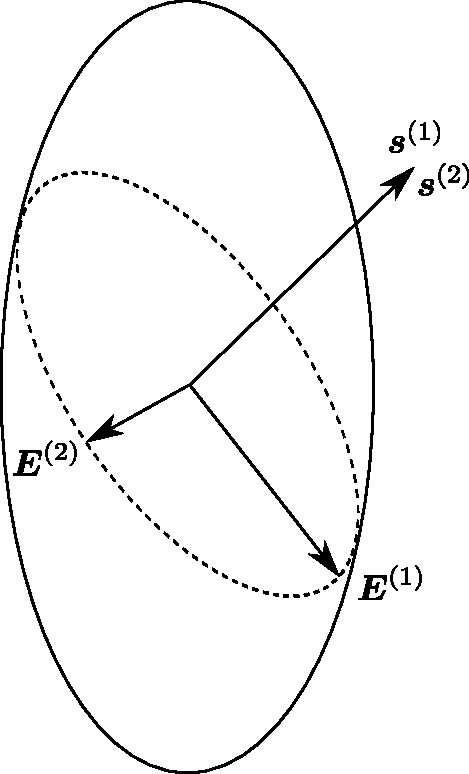
\includegraphics[scale=0.4]{fEllipse.pdf}
  \caption{Fresnel楕円体}
  \label{fEllipse}
\end{figure}

また,先程と同様の議論から,Fresnel楕円体を中心を通り$\boldsymbol{s}$に垂直な面で切った時の楕円断面の長半径及び短半径は2つの光線ベクトルの大きさ$s^{(1)}$, $s^{(2)}$に等しく,
各半径のベクトルは電場$\boldsymbol{E}^{(1)}$, $\boldsymbol{E}^{(2)}$の向きを向いていることが分かる.
また,誘電率が位置によって変化しない均質な物質では,$\boldsymbol{s}$と$\boldsymbol{n}$は変化しないので,2つの楕円体を光と共に動かして考えると,電束密度と電場の方向は常に同じ向きであることが分かる.
つまり,異方性媒質中を伝わる2つの光は直線偏光であることが分かる.

最後に異方性媒質を伝播する光波の重要な性質をいくらかまとめておく.
\begin{enumerate}
  \item $\boldsymbol{E}$, $\boldsymbol{D}$, $\boldsymbol{k}(\boldsymbol{n})$, $\boldsymbol{S}(\boldsymbol{s})$は同一平面内に存在し,$\boldsymbol{H}$はそれに直交する.
  \item 群速度(光線ベクトル)とPoyntingベクトルは同じ向きを向いている.つまり,群速度の向きにエネルギーの伝播が起こっている.
  \item 向きが決まっている群速度(光線ベクトル),波数(屈折率ベクトル)についてはその絶対値が2つ存在する.
  \item (実空間において)屈折率ベクトルは等位相面に直交する.
  \item 光線ベクトルはFresnel方程式から決定される屈折率ベクトル面の法線の向きを向いている.
  % ただし,屈折率ベクトル面は$(n_\xi,n_\eta,n_\zeta)$空間に存在する.
  \item 空間座標において原点から伸ばした光線ベクトルが作る面は等位相面である.
  \item 屈折率ベクトルは光線速度面方程式から決定される光線速度面の法線の向きを向いている.
  % ただし,光線速度面は$(s_\xi,s_\eta,s_\zeta)$空間に存在する.
  \item 同じ向きの屈折率ベクトルを持つ2つの光波の電束密度は直交する.
  \item 同じ向きの光線ベクトルを持つ2つの光波の電場は直交する.
  \item 実空間の屈折率楕円体によって2つの屈折率ベクトルの大きさと電束密度の向きが分かる.
  \item 実空間のFresnel楕円体によって2つの光線ベクトルの大きさと電場の向きが分かる.
  \item 異方性媒質中を伝わる2つの光は直線偏光である
\end{enumerate}

\paragraph{複屈折(1軸性結晶)}
1軸異方性の場合を考えよう.1軸性結晶には菱面体晶系,正方晶系,六方晶系などがある.
光学軸を$\zeta$軸とし,
\begin{align}
  \varepsilon=
  \begin{pmatrix}
    \varepsilon_{\text T} & 0 & 0\\
    0 & \varepsilon_{\text T} & 0\\
    0 & 0 & \varepsilon_{\text P}
  \end{pmatrix}
  \label{uniaxial_tensor1}
\end{align}
とする.この時,Fresnel方程式は因数分解され,
\begin{align}
  \dfrac{1}{\varepsilon_0}=\mu{c}^2&=\dfrac{n^2}{\varepsilon_{\text T}}\label{uniaxial_ordinary}\\
  \dfrac{1}{\varepsilon_0}=\mu{c}^2&=\dfrac{{n_\xi}^2+{n_\eta}^2}{\varepsilon_{\text P}}+\dfrac{{n_\zeta}^2}{\varepsilon_{\text T}}\label{uniaxial_extraordinary}
\end{align}
となる.(\ref{uniaxial_ordinary})を常光線,(\ref{uniaxial_extraordinary})を異常光線と言う.
Fresnel方程式は$(n_\xi,n_\eta,n_\zeta)$空間において,4次曲面を描くのであった.
これが因数分解されるといことは,曲面が2つ存在するということである.
それらが常光線と異常光線である.
常光線(\ref{uniaxial_ordinary})は球を,異常光線(\ref{uniaxial_extraordinary})は回転楕円体を表す.
これらを図示すると,以下のようになる($\varepsilon_{\text T}$と$\varepsilon_{\text P}$の大小で2通りに分かれる).

\begin{figure}[ht]
  \centering
  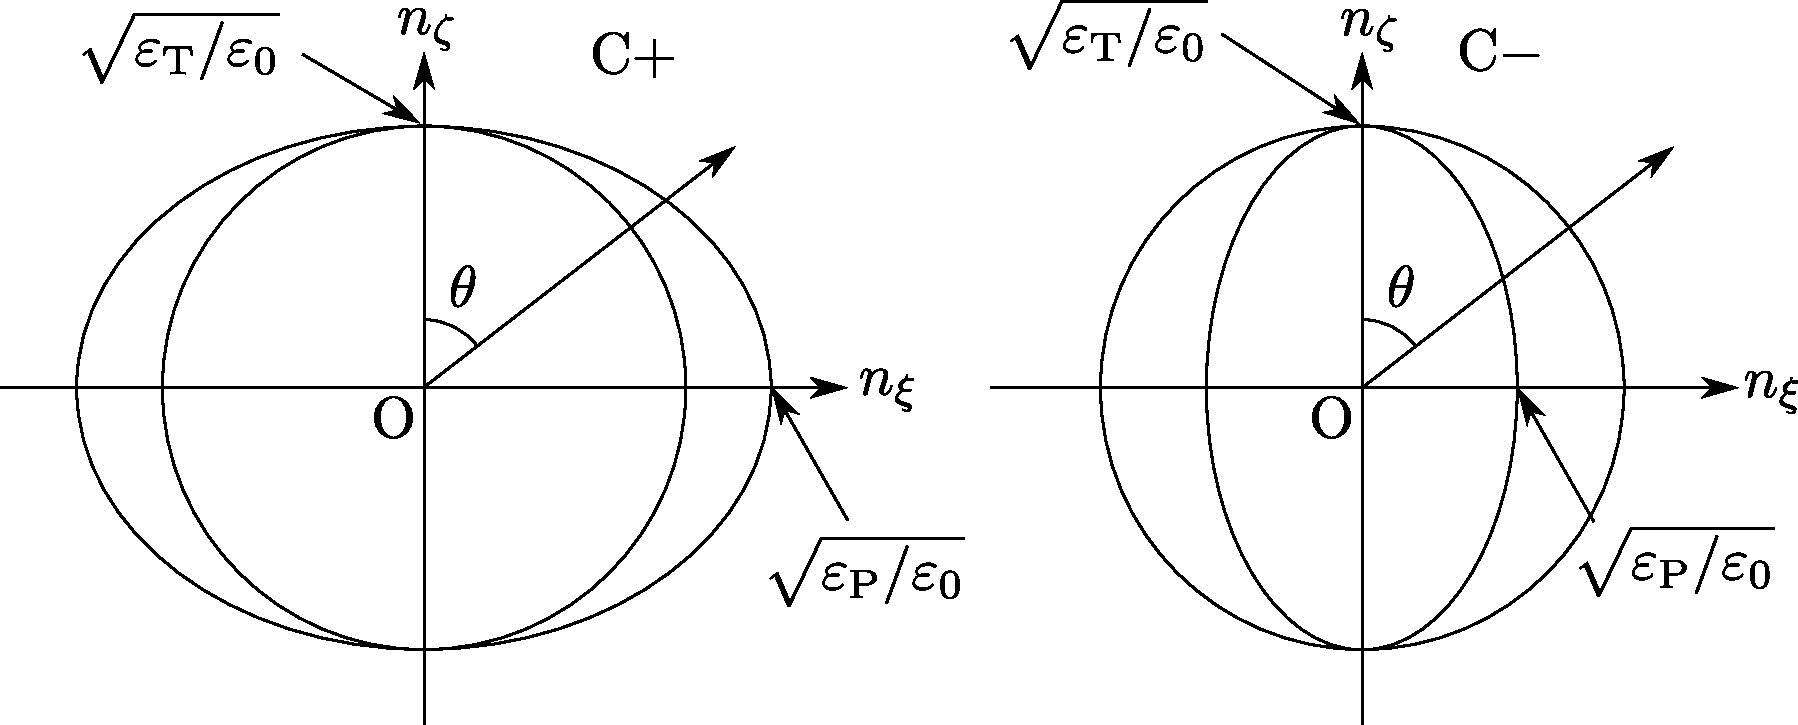
\includegraphics[scale=0.35]{uniaxiNvec.pdf}
  \caption{正結晶(左)と負結晶(右)}
  \label{uniaxiNvec}
\end{figure}

正結晶には水晶,氷;負結晶には方解石,ADPなどがある.
中心から$\boldsymbol{n}$の方向に引いた線分と曲面の交点が2つの屈折率ベクトルとなる.
異方性媒質一般で見たように,
光線ベクトルはFresnel方程式から決定される屈折率ベクトル面の法線の向きを向いているのであった.
なので,常光線においては$\boldsymbol{s}$と$\boldsymbol{n}$の向きは一致する.これは$\boldsymbol{E}$と$\boldsymbol{D}$の向きも一致するということである.
\eqref{aniso_newD}からも分かるように,
\begin{align}
  \boldsymbol{D}=\dfrac{1}{\mu{c^2}}n^2\boldsymbol{E}=\varepsilon_{\text T}\boldsymbol{E}
\end{align}
となる.つまり,
常光線は等方的な誘電率$\varepsilon_{\text T}$を持つ媒質中の光と同じように振る舞うことが分かる.

異常光線においても,光線ベクトルは屈折率ベクトル面の法線の向きを向いていることを考慮すると,
光線ベクトル$\boldsymbol{s}$は光学軸と屈折率ベクトル$\boldsymbol{n}$を通る平面(主断面)内に存在することが分かる.
$\boldsymbol{n}$が光学軸となす角を$\theta$とすると,(\ref{uniaxial_extraordinary})から,
\begin{align}
  \dfrac{1}{n^2}=\dfrac{\varepsilon_0}{\varepsilon_{\text P}}\sin^2\theta+\dfrac{\varepsilon_0}{\varepsilon_{\text T}}\cos^2\theta
\end{align}
となる.簡単のため,$\boldsymbol{n}$が$\xi\zeta$平面に存在するものとする.
この時,半直線と楕円の交点における法線の方向(光線ベクトルの向きに等しい)は,
\[\left(\dfrac{\tan\theta}{\varepsilon_{\text P}},0,\dfrac{1}{\varepsilon_{\text T}}\right)\]
となる.光線ベクトルが光学軸となす角$\theta'$は一般の場合に戻して考えても結局,
\begin{align}
  \tan\theta'=\dfrac{\varepsilon_{\text T}}{\varepsilon_{\text P}}\tan\theta\label{uniaxial_sandn}
\end{align}
である.$\boldsymbol{n}$が$\boldsymbol{s}$と同じ向きを向くのは,光学軸に平行に伝わる場合か,垂直に伝わる場合のみである.

以上の事実を踏まえれば常光線と以上光線の電場と磁場,そして磁束密度の位置関係が分かる.
異方性媒質中では2つの光波は直線偏光であることに注意.
まずは屈折率楕円体を考えよう.
この座標系では,屈折率楕円体は回転楕円体となる.それは次に示すようになる.

\begin{figure}[ht]
  \centering
  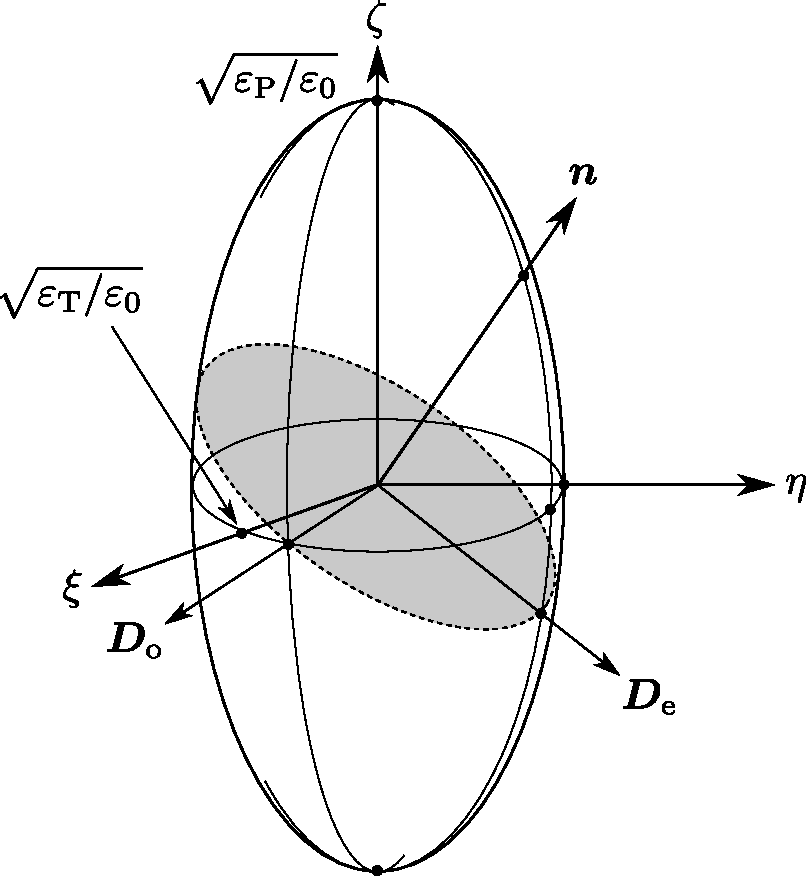
\includegraphics[scale=0.4]{uniaxial_nEllipse.pdf}
  \caption{常光線と異常光線の電束密度を示す屈折率楕円体(正結晶)}
  \label{uniaxial_nEllipse}
\end{figure}

以後,断りがないかぎり常光線の物理量を添字$_{\text o}$,異常光線の物理量を添字$_{\text e}$で表す.
屈折率楕円体からは2つの電束密度が存在することしか分からないが,(\ref{uniaxial_ordinary})を見れば,楕円の主半径のうち,$\zeta=0$に存在する方が常光線だと分かる.
以上の考察から重要な結果が得られた.
まず,常光線の電束密度は$\xi\eta$平面上に存在するということである.
もう一つが異常光線ベクトルの電束密度は主断面上に存在するということである.
常光線においては光は誘電率$\varepsilon_{\text T}$の等方的な媒質中と同じように振舞うので,常光線の電場は$\xi\eta$平面に存在することが分かる.
さらに,$\boldsymbol{E},\boldsymbol{D},\boldsymbol{s},\boldsymbol{n}$は同一平面内に存在するので,異常光線の電場は主断面上に存在することが分かる.
磁場の方向については,$\boldsymbol{H}=\dfrac{1}{\omega\mu}\boldsymbol{n}\times\boldsymbol{E}$から簡単に導くことができよう.

以上から,常光線と異常光線の電場と磁場の方向を図示すると本文図8-13のようになる.

1軸性の異方性を持つ媒質中では光はこのように進む.この2つの光は直線偏光である.

これまでは異方的な媒質の中のみを進む光を考えてきた.ここで,異方的な媒質に入る光について考えてみよう.
境界面を$y=0$,光学軸を$z$軸に取る.入射前の$\boldsymbol{n}$は$yz$平面に存在していたとする.
真空中から角度$\theta$で入射した光は異方性媒質に入ると常光線と異常光線に分かれる.
常光線の屈折角$\theta$は
\begin{align}
  \sqrt{\varepsilon_0}\sin\theta=\sqrt{\varepsilon_{\text T}}\sin\theta_{\text o}\label{uniaxial_refo}
\end{align}
で与えられる.異常光線の屈折角は(\ref{uniaxial_extraordinary})と(\ref{uniaxial_sandn})から,
\begin{align}
  \tan\theta_{\text e}=\sqrt{\dfrac{\varepsilon_{\text P}\varepsilon_0}{\varepsilon_{\text T}\left(\varepsilon_{\text T}-\varepsilon_0\sin^2\theta\right)}}\sin\theta\label{uniaxial_refe}
\end{align}
で与えられる.我々が光の進む向きとして観測するのは波数や位相速度の向きでなく,群速度の向きである.
(\ref{uniaxial_refo})と(\ref{uniaxial_refe})から,常光線と異常光線は屈折角が異なる.
そのため,1軸性異方性媒質を特定の条件で通った光は,別々の光線に分かれる.これを複屈折と呼ぶ.

\paragraph{円錐屈折(2軸性結晶)}
2軸性異方性媒質ではテンソル$\varepsilon$の主値は全て異なる.2軸性結晶には三斜晶系,単斜晶系,菱面体晶系などがある.
以下では,テンソルの主値を
\begin{align}
  \varepsilon_\xi < \varepsilon_\eta < \varepsilon_\zeta\label{biaxial_nlarge}
\end{align}
とする.このようにしても一般性を失わないことは明らかである.
Fresnel方程式は,
\begin{align}
  n^2\left(\varepsilon_{\xi}{n_\xi}^2+\varepsilon_{\eta}{n_\eta}^2+\varepsilon_{\zeta}{n_\zeta}^2\right)
  -\mu{c}^2\left[{n_\xi}^2\varepsilon_\xi(\varepsilon_\eta+\varepsilon_\zeta)
  +{n_\eta}^2\varepsilon_\eta(\varepsilon_\zeta+\varepsilon_\xi)
  +{n_\zeta}^2\varepsilon_\zeta(\varepsilon_\eta+\varepsilon_\xi)\right]
  +\mu^2{c}^4\varepsilon_\xi\varepsilon_\eta\varepsilon_\zeta=0\label{biaxial_fresEq}
\end{align}
のように書けるのであった.まずはこの4次曲面,つまり屈折率ベクトル面の形状を求めよう.
$n_\xi{}n_\eta$平面での切り口は,(\ref{biaxial_fresEq})に$n_\zeta=0$を代入して,
\[\left(n^2-\mu{c^2}\varepsilon_\zeta\right)\left(\varepsilon_\xi{n_\xi}^2+\varepsilon_\eta{n_\eta}^2-\mu{c^2}\varepsilon_\xi\varepsilon_\eta\right)=0\]
より,円
\begin{align}
  \dfrac{{n_\xi}^2}{\varepsilon_\zeta/\varepsilon_0}+\dfrac{{n_\eta}^2}{\varepsilon_\zeta/\varepsilon_0}=1
\end{align}
及び楕円
\begin{align}
  \dfrac{{n_\xi}^2}{\varepsilon_\eta/\varepsilon_0}+\dfrac{{n_\eta}^2}{\varepsilon_\xi/\varepsilon_0}=1
\end{align}
となる.(\ref{biaxial_nlarge})の条件から,楕円は円の内側にあることが分かる.
同様に計算すると,
\begin{align}
  \dfrac{{n_\eta}^2}{\varepsilon_\xi/\varepsilon_0}+\dfrac{{n_\zeta}^2}{\varepsilon_\xi/\varepsilon_0}=1\\
  \dfrac{{n_\eta}^2}{\varepsilon_\zeta/\varepsilon_0}+\dfrac{{n_\zeta}^2}{\varepsilon_\eta/\varepsilon_0}=1\\
  \dfrac{{n_\zeta}^2}{\varepsilon_\eta/\varepsilon_0}+\dfrac{{n_\xi}^2}{\varepsilon_\eta/\varepsilon_0}=1\label{biaxial_xzc}\\
  \dfrac{{n_\zeta}^2}{\varepsilon_\xi/\varepsilon_0}+\dfrac{{n_\xi}^2}{\varepsilon_\zeta/\varepsilon_0}=1\label{biaxial_xze}
\end{align}
が得られる.これらを図示すると,次のようになる.

\begin{figure}[ht]
  \centering
  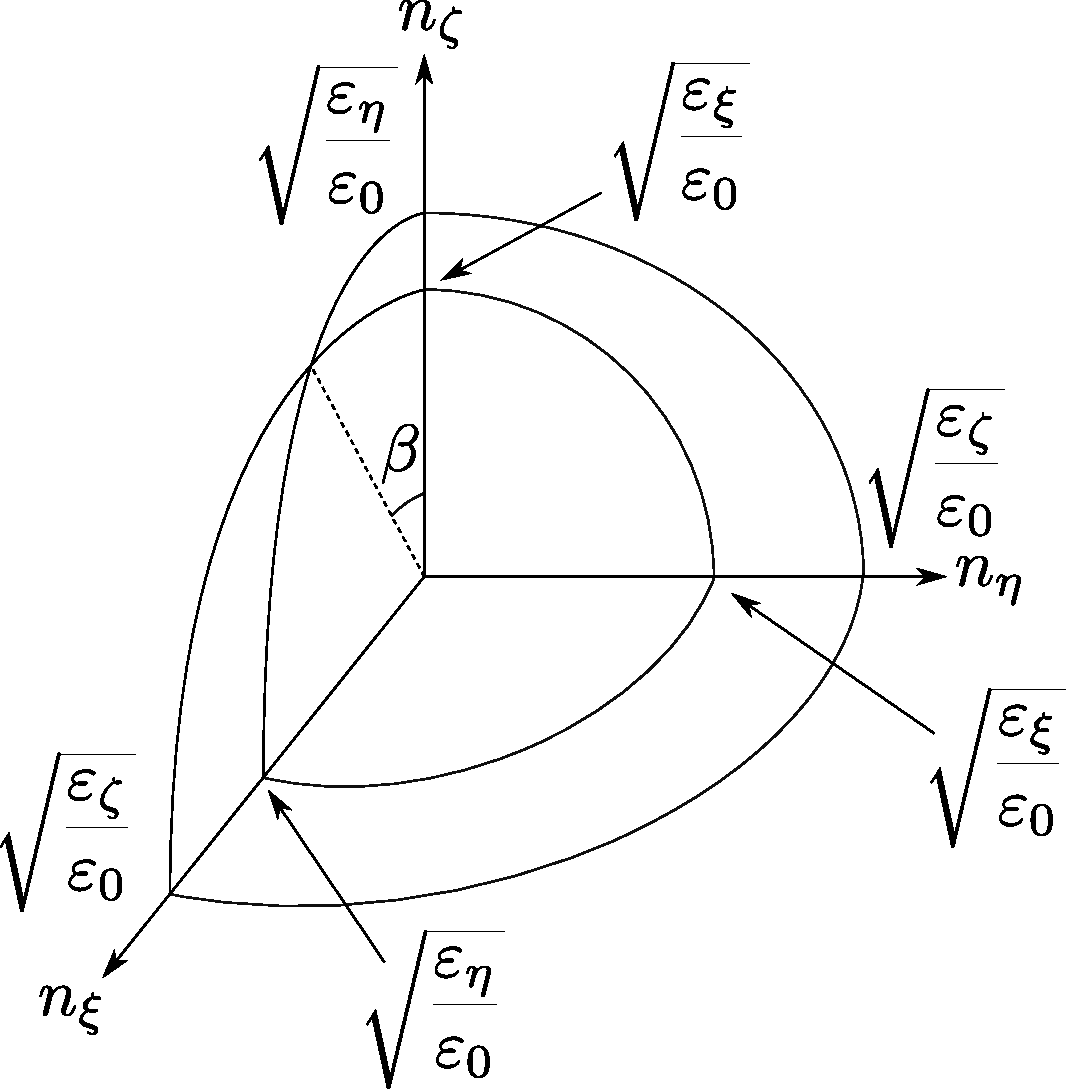
\includegraphics[scale=0.35]{fresnel.pdf}
  \caption{}
  \label{fresnel}
\end{figure}

この曲面は自身との交点を4つ持っており,それらは$n_\xi{}n_\zeta$平面の各象限に存在する.
特異点の傾き$\beta$は,(\ref{biaxial_xzc})と(\ref{biaxial_xze})から,
\begin{align}
  \tan\beta=\pm\sqrt{\dfrac{\varepsilon_\zeta(\varepsilon_\eta-\varepsilon_\xi)}{\varepsilon_\xi(\varepsilon_\zeta-\varepsilon_\eta)}}\label{biaxial_betat}\\
  \cos\beta=\pm\sqrt{\dfrac{\varepsilon_\xi(\varepsilon_\zeta-\varepsilon_\eta)}{\varepsilon_\eta(\varepsilon_\zeta-\varepsilon_\xi)}}\label{biaxial_betac}\\
  \sin\beta=\pm\sqrt{\dfrac{\varepsilon_\zeta(\varepsilon_\eta-\varepsilon_\xi)}{\varepsilon_\eta(\varepsilon_\zeta-\varepsilon_\xi)}}\label{biaxial_betas}
\end{align}
で与えられる.この式により,$n_\xi{}n_\zeta$平面上に2本の軸が決定される.
2軸性異方性媒質ではこの軸のことを光学軸もしくは双法線と呼ぶ.
光学軸の方向は,波動ベクトルの絶対値が一つの値しか取らない,つまりFresnel方程式が重解を持つ方向である.
また,$n$の値が1つに定まることから,光学軸の向きで屈折率楕円体を切断すると断面は円となる.

光線ベクトルと光線速度面についても同様の式が成り立つ.
光線速度面方程式は,
\begin{align}
  s^2\left(\varepsilon_\eta\varepsilon_\zeta{s_\xi}^2 + \varepsilon_\zeta\varepsilon_\xi{s_\eta}^2 + \varepsilon_\xi\varepsilon_\eta{s_\zeta}^2\right)
  -\dfrac{1}{\mu{}c^2}\left[{s_\xi}^2(\varepsilon_\eta+\varepsilon_\zeta)+{s_\eta}^2(\varepsilon_\zeta+\varepsilon_\xi)+{s_\zeta}^2(\varepsilon_\xi+\varepsilon_\eta)\right]
  +\dfrac{1}{\mu^2c^4}=0
\end{align}
で与えられるのであった.これも,$s$座標系で4次曲面をなす.特異点が$\zeta$軸となす角を$\gamma$とする.
\begin{align}
  \dfrac{{s_\zeta}^2}{\varepsilon_0/\varepsilon_\eta}+\dfrac{{s_\xi}^2}{\varepsilon_0/\varepsilon_\eta}=1\label{biaxial_szxc}\\
  \dfrac{{s_\zeta}^2}{\varepsilon_0/\varepsilon_\xi}+\dfrac{{s_\xi}^2}{\varepsilon_0/\varepsilon_\zeta}=1\label{biaxial_szxe}
\end{align}
から,
\begin{align}
  \tan\gamma=\pm\sqrt{\dfrac{\varepsilon_\eta-\varepsilon_\xi}{\varepsilon_\zeta-\varepsilon_\eta}}=\sqrt{\dfrac{\varepsilon_\zeta}{\varepsilon_\xi}}\tan\beta\label{biaxial_gamma}
\end{align}
となる.最後の式変形には(\ref{biaxial_betat})を使った.この$\gamma$で決定される2本の軸を光線軸もしくは双径線と呼ぶ.
また,$s$の値が1つに定まることから,光線軸の向きでFresnel楕円体を切断すると断面は円となる.
さらに,(\ref{biaxial_nlarge}),(\ref{biaxial_gamma})から,
\begin{align}
  \gamma < \beta
\end{align}
であることが分かる.

異方性媒質一般で調べたように,$\boldsymbol{s}$は屈折率ベクトル面の法線方向を向くのであった.
つまり,
\begin{align}
  \dfrac{\partial f}{\partial\boldsymbol{n}}\parallel\boldsymbol{s}\label{biaxial_fns}
\end{align}
である.(\ref{biaxial_fresEq})から,
\begin{align}
  \begin{split}
    An_\xi\left[\mu{c^2}\varepsilon_\xi(\varepsilon_\eta+\varepsilon_\zeta)-\varepsilon_\xi{n^2}-(\varepsilon_{\xi}{n_\xi}^2+\varepsilon_{\eta}{n_\eta}^2+\varepsilon_{\zeta}{n_\zeta}^2)\right]=s_\xi\\
    An_\eta\left[\mu{c^2}\varepsilon_\eta(\varepsilon_\zeta+\varepsilon_\xi)-\varepsilon_\eta{n^2}-(\varepsilon_{\xi}{n_\xi}^2+\varepsilon_{\eta}{n_\eta}^2+\varepsilon_{\zeta}{n_\zeta}^2)\right]=s_\eta\\
    An_\zeta\left[\mu{c^2}\varepsilon_\zeta(\varepsilon_\xi+\varepsilon_\eta)-\varepsilon_\zeta{n^2}-(\varepsilon_{\xi}{n_\xi}^2+\varepsilon_{\eta}{n_\eta}^2+\varepsilon_{\zeta}{n_\zeta}^2)\right]=s_\zeta
  \end{split}\label{biaxial_ns}
\end{align}
となれば良い.ただし,$A$は0でない定数である.
$\boldsymbol{s}$と$\boldsymbol{n}$が平行になるのは,誘電主軸の向きに伝播する時のみだと分かる.
$\boldsymbol{s}$は群速度の向きを向いていて,大きさが$\boldsymbol{s}\cdot\boldsymbol{n}=1$で決定されるのであった.(\ref{biaxial_ns})から,
\begin{align*}
  & A{n_\xi}^2\left[\mu{c^2}\varepsilon_\xi(\varepsilon_\eta+\varepsilon_\zeta)-\varepsilon_\xi{n^2}-(\varepsilon_{\xi}{n_\xi}^2+\varepsilon_{\eta}{n_\eta}^2+\varepsilon_{\zeta}{n_\zeta}^2)\right]\\
  &+ A{n_\eta}^2\left[\mu{c^2}\varepsilon_\eta(\varepsilon_\zeta+\varepsilon_\xi)-\varepsilon_\eta{n^2}-(\varepsilon_{\xi}{n_\xi}^2+\varepsilon_{\eta}{n_\eta}^2+\varepsilon_{\zeta}{n_\zeta}^2)\right]\\
  &+ A{n_\zeta}^2\left[\mu{c^2}\varepsilon_\zeta(\varepsilon_\xi+\varepsilon_\eta)-\varepsilon_\zeta{n^2}-(\varepsilon_{\xi}{n_\xi}^2+\varepsilon_{\eta}{n_\eta}^2+\varepsilon_{\zeta}{n_\zeta}^2)\right]=1
\end{align*}
となるので,これを解くと,
\begin{align}
  A=\dfrac{\varepsilon_0}{{n_\xi}^2\varepsilon_\xi\left(\varepsilon_\eta+\varepsilon_\zeta\right)+{n_\eta}^2\varepsilon_\eta\left(\varepsilon_\zeta+\varepsilon_\xi\right)+{n_\zeta}^2\varepsilon_\zeta\left(\varepsilon_\xi+\varepsilon_\eta\right)-2\varepsilon_0n^2\left(\varepsilon_{\xi}{n_\xi}^2+\varepsilon_{\eta}{n_\eta}^2+\varepsilon_{\zeta}{n_\zeta}^2\right)}
\end{align}
となる.(\ref{biaxial_ns})に代入すると,
\begin{align}
  \begin{split}
    s_\xi=\dfrac{n_\xi\left[\varepsilon_\xi(\varepsilon_\eta+\varepsilon_\zeta)-\varepsilon_0\varepsilon_\xi{n^2}-\varepsilon_0(\varepsilon_{\xi}{n_\xi}^2+\varepsilon_{\eta}{n_\eta}^2+\varepsilon_{\zeta}{n_\zeta}^2)\right]}
    {{n_\xi}^2\varepsilon_\xi\left(\varepsilon_\eta+\varepsilon_\zeta\right)+{n_\eta}^2\varepsilon_\eta\left(\varepsilon_\zeta+\varepsilon_\xi\right)+{n_\zeta}^2\varepsilon_\zeta\left(\varepsilon_\xi+\varepsilon_\eta\right)-2\varepsilon_0n^2\left(\varepsilon_{\xi}{n_\xi}^2+\varepsilon_{\eta}{n_\eta}^2+\varepsilon_{\zeta}{n_\zeta}^2\right)}\\
    %
    s_\eta=\dfrac{n_\eta\left[\varepsilon_\eta(\varepsilon_\zeta+\varepsilon_\xi)-\varepsilon_0\varepsilon_\eta{n^2}-\varepsilon_0(\varepsilon_{\xi}{n_\xi}^2+\varepsilon_{\eta}{n_\eta}^2+\varepsilon_{\zeta}{n_\zeta}^2)\right]}
    {{n_\xi}^2\varepsilon_\xi\left(\varepsilon_\eta+\varepsilon_\zeta\right)+{n_\eta}^2\varepsilon_\eta\left(\varepsilon_\zeta+\varepsilon_\xi\right)+{n_\zeta}^2\varepsilon_\zeta\left(\varepsilon_\xi+\varepsilon_\eta\right)-2\varepsilon_0n^2\left(\varepsilon_{\xi}{n_\xi}^2+\varepsilon_{\eta}{n_\eta}^2+\varepsilon_{\zeta}{n_\zeta}^2\right)}\\
    %
    s_\zeta=\dfrac{n_\zeta\left[\varepsilon_\zeta(\varepsilon_\xi+\varepsilon_\eta)-\varepsilon_0\varepsilon_\zeta{n^2}-\varepsilon_0(\varepsilon_{\xi}{n_\xi}^2+\varepsilon_{\eta}{n_\eta}^2+\varepsilon_{\zeta}{n_\zeta}^2)\right]}
    {{n_\xi}^2\varepsilon_\xi\left(\varepsilon_\eta+\varepsilon_\zeta\right)+{n_\eta}^2\varepsilon_\eta\left(\varepsilon_\zeta+\varepsilon_\xi\right)+{n_\zeta}^2\varepsilon_\zeta\left(\varepsilon_\xi+\varepsilon_\eta\right)-2\varepsilon_0n^2\left(\varepsilon_{\xi}{n_\xi}^2+\varepsilon_{\eta}{n_\eta}^2+\varepsilon_{\zeta}{n_\zeta}^2\right)}
  \end{split}
  \label{biaxial_ncomp}
\end{align}
が得られる.$\boldsymbol{n}$が双法線の向きを向いている場合を考えよう.この時,$\boldsymbol{n}$は曲面$f=0$の特異点を通る.
この方程式はこの点において重解をもつので,特異点における$\dfrac{\partial{f}}{\partial{n_i}}$は0である.
この時,(\ref{biaxial_ncomp})は$0/0$の不定形になる.よって,双法線方向に進む光については別に考え直す必要がある.

まずは,ある座標系に屈折率ベクトル面と光線速度面を作ろう(これらはFresnel方程式,光線速度面方程式から決定され,異なる座標系に属するものだが,適当な目盛で両者の空間を一致させたとする).
これを今までに習い$(\xi,\eta,\zeta)$空間とし,$\xi\eta$平面を図示すると次のようになる(屈折率ベクトル面を考える際は$i\to{}n_i$,光線速度面を考える際は$i\to{}s_i$と書き換える).

\begin{figure}[ht]
  \centering
  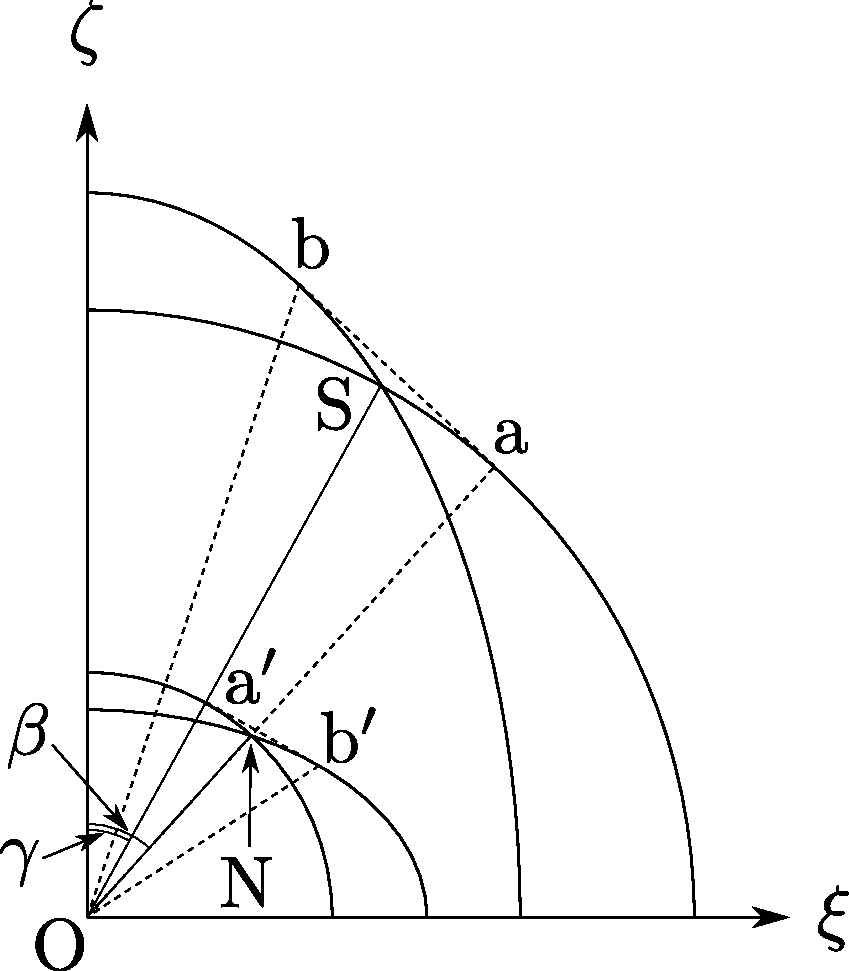
\includegraphics[scale=0.35]{biaxinands.pdf}
  \caption{}
  \label{biaxinands}
\end{figure}

まずは光線速度面Sに2点で接する直線abを求めよう.(\ref{biaxial_betat}),(\ref{biaxial_szxc}),(\ref{biaxial_szxe})から,これは
\begin{align}
  s_\xi\sin\beta+s_\zeta\cos\beta=\sqrt{\dfrac{\varepsilon_0}{\varepsilon_\eta}}
\end{align}
となる.さらにOaが$\zeta$軸となす角は,aが半径$\sqrt{\varepsilon_0/\varepsilon_\eta}$の円周上だということを考えると,$\beta$である.
よって,屈折率ベクトル面の特異点Nと原点を通る直線と光線速度面との交点は,光線速度面とある直線の接点であり,この直線は法線となる.
次に,これを三次元に拡張しよう.光線速度面の方程式は,
\begin{align}
  g & = \left({s_\xi}^2+{s_\eta}^2+{s_\zeta}^2\right)\left(\varepsilon_\eta\varepsilon_\zeta{s_\xi}^2+\varepsilon_\zeta\varepsilon_\xi{s_\eta}^2+\varepsilon_\xi\varepsilon_\eta{s_\zeta}^2\right) \notag \\
  &-{\varepsilon_0}\left[{s_\xi}^2(\varepsilon_\eta+\varepsilon_\zeta)+{s_\eta}^2(\varepsilon_\zeta+\varepsilon_\xi)+{s_\zeta}^2(\varepsilon_\xi+\varepsilon_\eta)\right]
  +{\varepsilon_0}^2=0\label{biaxial_g0}
\end{align}
である.さらに,これの$\boldsymbol{a}(\sqrt{\varepsilon_0/\varepsilon_\eta}\sin\beta,0,\sqrt{\varepsilon_0/\varepsilon_\eta}\cos\beta)$での接平面は,
\begin{align*}
  \dfrac{\partial{g}}{\partial\boldsymbol{s}}(\boldsymbol{a})\cdot(\boldsymbol{r}-\boldsymbol{a})=0
\end{align*}
で与えられる.$\dfrac{\partial{g}}{\partial\boldsymbol{s}}(\boldsymbol{a})$は,それぞれ
\begin{align}
  \dfrac{\partial{g}}{\partial{}s_\xi}(\boldsymbol{a}) &= 2\left[\varepsilon_\eta\varepsilon_\zeta{s_\xi}^2+\varepsilon_\zeta\varepsilon_\xi{s_\eta}^2+\varepsilon_\xi\varepsilon_\eta{s_\zeta}^2+\varepsilon_\eta\varepsilon_\zeta\left({s_\xi}^2+{s_\eta}^2+{s_\zeta}^2\right)-\varepsilon_0(\varepsilon_\eta+\varepsilon_\zeta)\right]s_\xi(\boldsymbol{a})\notag\\
  &= 2\left[\varepsilon_\eta\varepsilon_\zeta{s_\xi}^2+\varepsilon_\zeta\varepsilon_\xi{s_\eta}^2+\varepsilon_\xi\varepsilon_\eta{s_\zeta}^2-\varepsilon_0\varepsilon_\eta\right]s_\xi(\boldsymbol{a})\\
  \dfrac{\partial{g}}{\partial{}s_\xi}(\boldsymbol{a}) &= 2\left[\varepsilon_\eta\varepsilon_\zeta{s_\xi}^2+\varepsilon_\zeta\varepsilon_\xi{s_\eta}^2+\varepsilon_\xi\varepsilon_\eta{s_\zeta}^2+\varepsilon_\zeta\varepsilon_\xi\left({s_\xi}^2+{s_\eta}^2+{s_\zeta}^2\right)-\varepsilon_0(\varepsilon_\zeta+\varepsilon_\xi)\right]s_\eta(\boldsymbol{a})\notag\\
  &= 0\\
  \dfrac{\partial{g}}{\partial{}s_\xi}(\boldsymbol{a}) &= 2\left[\varepsilon_\eta\varepsilon_\zeta{s_\xi}^2+\varepsilon_\zeta\varepsilon_\xi{s_\eta}^2+\varepsilon_\xi\varepsilon_\eta{s_\zeta}^2+\varepsilon_\xi\varepsilon_\eta\left({s_\xi}^2+{s_\eta}^2+{s_\zeta}^2\right)-\varepsilon_0(\varepsilon_\xi+\varepsilon_\eta)\right]s_\zeta(\boldsymbol{a})\notag\\
  &= 2\left[\varepsilon_\eta\varepsilon_\zeta{s_\xi}^2+\varepsilon_\zeta\varepsilon_\xi{s_\eta}^2+\varepsilon_\xi\varepsilon_\eta{s_\zeta}^2-\varepsilon_0\varepsilon_\eta\right]s_\zeta(\boldsymbol{a})
\end{align}
となる.よって,平面の法線は$(\sin\beta,0,\cos\beta)$を向いている.結局,接平面も
\begin{align}
  \text{C} \colon s_\xi\sin\beta+s_\zeta\cos\beta=\sqrt{\dfrac{\varepsilon_0}{\varepsilon_\eta}}\label{biaxial_plane}
\end{align}
の形で表される.これは上の図ではabで表現されている.この形から分かるように,
Oaは接平面と直交することが分かる.
次にこの平面と曲面の他の接点を考えよう.曲面上の点$\boldsymbol{r}$が平面Cに接するには,(\ref{biaxial_g0}),(\ref{biaxial_plane})に加えて
\begin{align}
  \dfrac{\partial{g}}{\partial\boldsymbol{s}}(\boldsymbol{r})&\parallel(\sin\beta,0,\cos\beta)
\end{align}
であればよい.これらの条件から,接点は(\ref{biaxial_g0}),(\ref{biaxial_plane})及び
\begin{align}
  &\left[\varepsilon_\eta\varepsilon_\zeta{s_\xi}^2+\varepsilon_\zeta\varepsilon_\xi{s_\eta}^2+\varepsilon_\xi\varepsilon_\eta{s_\zeta}^2+\varepsilon_\eta\varepsilon_\zeta\left({s_\xi}^2+{s_\eta}^2+{s_\zeta}^2\right)-\varepsilon_0(\varepsilon_\eta+\varepsilon_\zeta)\right]s_\xi\cos\beta\notag\\
  &\qquad=\left[\varepsilon_\eta\varepsilon_\zeta{s_\xi}^2+\varepsilon_\zeta\varepsilon_\xi{s_\eta}^2+\varepsilon_\xi\varepsilon_\eta{s_\zeta}^2+\varepsilon_\xi\varepsilon_\eta\left({s_\xi}^2+{s_\eta}^2+{s_\zeta}^2\right)-\varepsilon_0(\varepsilon_\xi+\varepsilon_\eta)\right]s_\zeta\sin\beta\label{biaxial_gxz}\\
  &\left[\varepsilon_\eta\varepsilon_\zeta{s_\xi}^2+\varepsilon_\zeta\varepsilon_\xi{s_\eta}^2+\varepsilon_\xi\varepsilon_\eta{s_\zeta}^2+\varepsilon_\zeta\varepsilon_\xi\left({s_\xi}^2+{s_\eta}^2+{s_\zeta}^2\right)-\varepsilon_0(\varepsilon_\zeta+\varepsilon_\xi)\right]s_\eta=0\label{biaxial_gy}
\end{align}
を満たさなければならない.(\ref{biaxial_gy})より,$s_\eta\neq0$では,$s_\eta$の係数が0でなくてはならない.よって,
\begin{align}
  \varepsilon_\zeta(\varepsilon_\xi+\varepsilon_\eta){s_\xi}^2+2\varepsilon_\zeta\varepsilon_\xi{s_\eta}^2+\varepsilon_\xi(\varepsilon_\eta+\varepsilon_\zeta){s_\zeta}^2=\varepsilon_0(\varepsilon_\zeta+\varepsilon_\xi)\label{biaxial_cnd1}
\end{align}
(\ref{biaxial_cnd1})は楕円体を表している.これと(\ref{biaxial_plane})の共通部分が解となるので,解は円を描く.
簡単のため,
\begin{align}
  A=\dfrac{\varepsilon_\zeta(\varepsilon_\xi+\varepsilon_\eta)}{\varepsilon_0(\varepsilon_\zeta+\varepsilon_\xi)},\quad
  B=\dfrac{2\varepsilon_\xi\varepsilon_\zeta}{\varepsilon_0(\varepsilon_\zeta+\varepsilon_\xi)},\quad
  C=\dfrac{\varepsilon_\xi(\varepsilon_\eta+\varepsilon_\zeta)}{\varepsilon_0(\varepsilon_\zeta+\varepsilon_\xi)}\label{biaxial_ABC}
\end{align}
としよう.まずは$s_\eta$軸に関して$\beta$だけ回転させる.回転後の方程式では,
\begin{align}
  \begin{split}
    s_\xi\to{}s_\xi\cos\beta+s_\zeta\sin\beta\\
    s_\zeta\to{}s_\zeta\cos\beta-s_\xi\sin\beta
  \end{split}
\end{align}
とすればよい.これから,楕円体(\ref{biaxial_cnd1})と平面(\ref{biaxial_plane})は
\begin{align}
  \left(A\cos^2\beta+C\sin^2\beta\right){s_\xi}^2+B{s_\eta}^2+\left(A\sin^2\beta+C\cos^2\beta\right){s_\zeta}^2+2(A-C)\cos\beta\sin\beta{}s_\xi{}s_\zeta =1\label{biaxial_ellipserot} \\
  \zeta =\sqrt{\dfrac{\varepsilon_0}{\varepsilon_\eta}}\label{biaxial_planerot}
\end{align}
となる.(\ref{biaxial_planerot}),(\ref{biaxial_betac}),(\ref{biaxial_betas}),(\ref{biaxial_ABC})を(\ref{biaxial_ellipserot})に代入して,解は
\begin{align}
  {s_\xi}^2+\sqrt{\dfrac{\varepsilon_0(\varepsilon_\zeta-\varepsilon_\eta)(\varepsilon_\eta-\varepsilon_\xi)}{\varepsilon_\xi\varepsilon_\eta\varepsilon_\zeta}}s_\xi+{s_\eta}^2=0 , \quad
  s_\zeta=\sqrt{\dfrac{\varepsilon_0}{\varepsilon_\eta}}
\end{align}
と求まる.よって,光線速度面と接平面の共通部分は円を描くことが分かる.
よって,もとの座標系においても半径$\dfrac{1}{2}\sqrt{\dfrac{\varepsilon_0(\varepsilon_\zeta-\varepsilon_\eta)(\varepsilon_\eta-\varepsilon_\xi)}{\varepsilon_\xi\varepsilon_\eta\varepsilon_\zeta}}$の円を描くことが分かる.
次に,この円と中心を結んで斜円錐(頂点から下した垂線の足と底面の円の中心が一致しない円錐)面を作ろう.

\begin{figure}[ht]
  \centering
  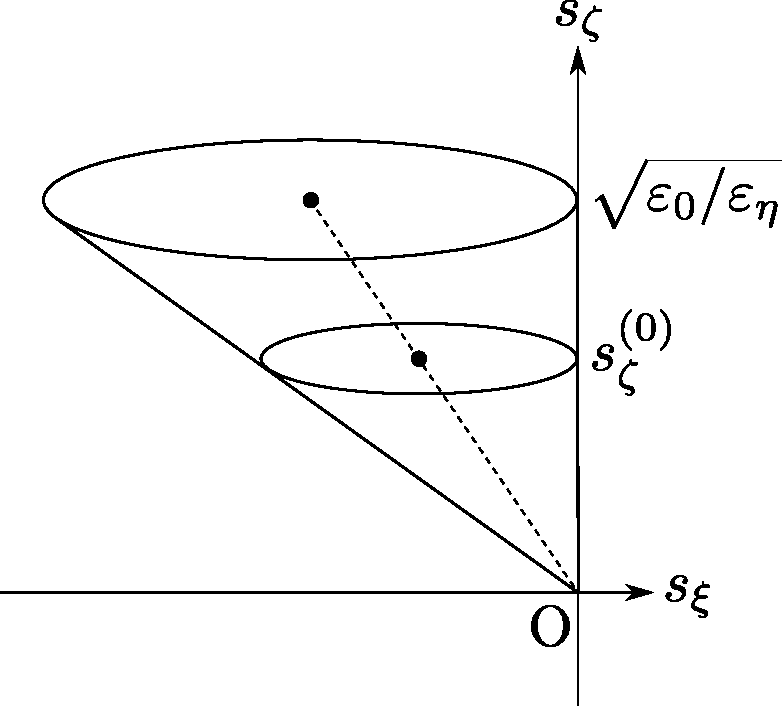
\includegraphics[scale=0.4]{scorn.pdf}
  \caption{}
  \label{scorn}
\end{figure}

% 直円錐(頂点から下した垂線の足と底面の円の中心が一致する円錐)を斜めに切って楕円が出てくるのとは別の話である.
さらに,$s$空間における点が実空間においてはベクトルになるように,$s$空間の平面は点$\boldsymbol{s}$の集合であり,実空間の平面になるとは限らないことに注意.
ある平面$s_\zeta=s_\zeta^{(0)}$でこの平面を切ると,これは底面と相似な円となり,$s_\zeta^{(0)}\sqrt{\varepsilon_\eta/\varepsilon_0}$倍になっている.
よって,円錐面の方程式は,
\begin{align*}
  \left(s_\xi+\dfrac{s_\zeta}{2}\sqrt{\dfrac{(\varepsilon_\zeta-\varepsilon_\eta)(\varepsilon_\eta-\varepsilon_\xi)}{\varepsilon_\xi\varepsilon_\zeta}}\right)^2+{s_\eta}^2=\left(\dfrac{s_\zeta}{2}\sqrt{\dfrac{(\varepsilon_\zeta-\varepsilon_\eta)(\varepsilon_\eta-\varepsilon_\xi)}{\varepsilon_\xi\varepsilon_\zeta}}\right)^2 .
\end{align*}
展開すれば,
\begin{align}
  {s_\xi}^2+\sqrt{\dfrac{(\varepsilon_\zeta-\varepsilon_\eta)(\varepsilon_\eta-\varepsilon_\xi)}{\varepsilon_\xi\varepsilon_\zeta}}s_\xi{}s_\zeta+{s_\eta}^2=0 . \label{biaxial_cornrot}
\end{align}
これを$\eta$軸に関して$-\beta$回転させると元の円錐が得られ,その変換は
\begin{align}
  \begin{split}
    s_\xi \to s_\xi\cos\beta-s_\zeta\sin\beta , \\
    s_\zeta \to s_\zeta\cos\beta+s_\xi\sin\beta .
  \end{split}
\end{align}
である.これを(\ref{biaxial_cornrot})に適用して,
\begin{align}
  (\varepsilon_\zeta-\varepsilon_\xi){s_\eta}^2 +
  \left[s_\xi\sqrt{\varepsilon_\xi(\varepsilon_\zeta-\varepsilon_\eta)} - s_\zeta\sqrt{\varepsilon_\zeta(\varepsilon_\eta-\varepsilon_\xi)}\right]
  \left(s_\xi\sqrt{\dfrac{\varepsilon_\zeta-\varepsilon_\eta}{\varepsilon_\xi}}-s_\zeta\sqrt{\dfrac{\varepsilon_\eta-\varepsilon_\xi}{\varepsilon_\zeta}}\right) = 0\label{biaxial_corn}
\end{align}
となる.この円錐面を内部円錐と呼ぶ.$\boldsymbol{s}$は$s$空間においてこの内部円錐と光線速度面の交線である円上に存在する.

以上が定量的な説明であったが,次にこれを定性的に考えよう.$\boldsymbol{s}$から光線速度面を使って$\boldsymbol{n}$を作る方法を使う.

\begin{figure}[ht]
  \centering
  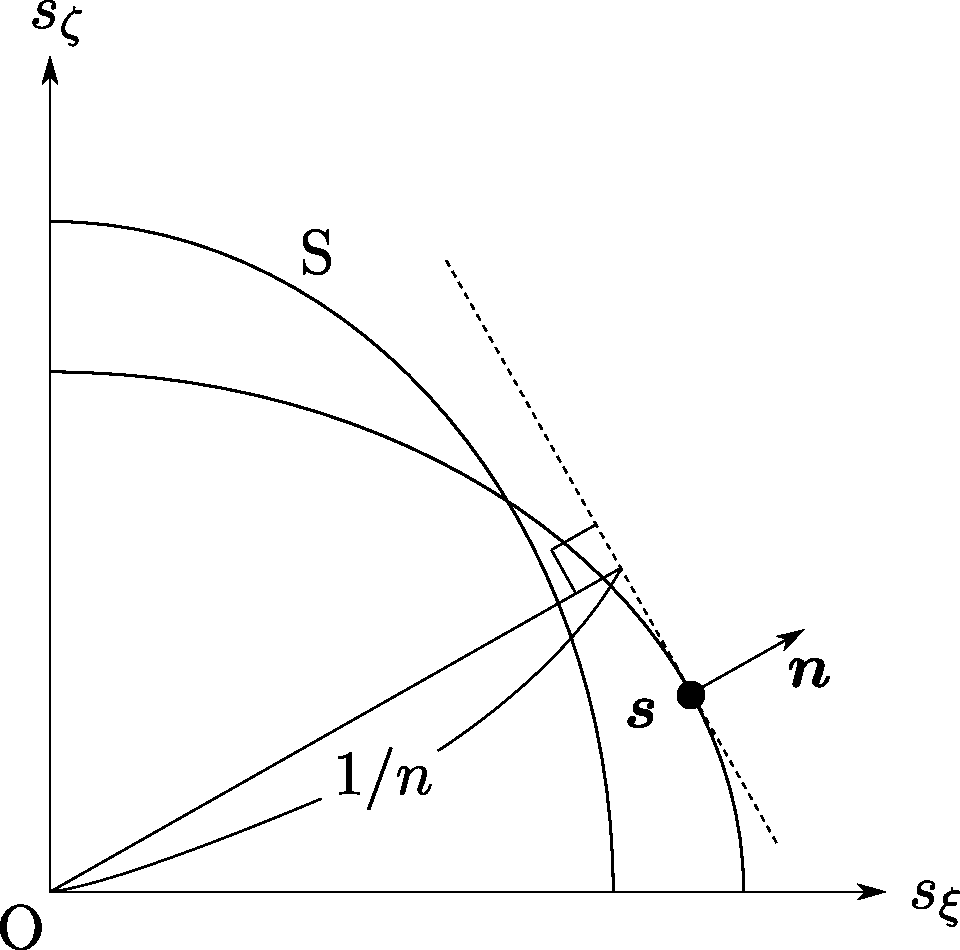
\includegraphics[scale=0.3]{ston.pdf}
  \caption{ $s$空間であることに注意}
  \label{ston}
\end{figure}

まず,ある$s$空間と光線ベクトル$\boldsymbol{s}$を考えよう.この空間内において$\boldsymbol{s}$は点として存在する.
今,媒質内のある点で$\boldsymbol{s}$が与えられた.この時,$s$空間に光線速度面方程式で決定される光線速度面Sを記入する.
そして,与えられた$\boldsymbol{s}$における法線を決定する.この法線の$s$空間における向きが屈折率ベクトル$\boldsymbol{n}$の実空間での向きと等しくなる.
図を見れば明らかなように,$\boldsymbol{s}$における光線速度面Sの接平面に原点から下した垂線はやはり$\boldsymbol{n}$の向きを向いている.
さらに,$\boldsymbol{s}\cdot\boldsymbol{n}$であることから,その長さは$\dfrac{1}{n}$である.

先程調べたように,2軸性異方性媒質の光線速度面上には同じ向きの法線を持つ領域が存在する.この点それぞれ$\boldsymbol{s}^{(1)}$, $\boldsymbol{s}^{(2)},\ldots$などと区別する.
ここで,任意の$\boldsymbol{s}^{(i)}$における接平面C$^{(i)}$を考える.この接平面は光線ベクトルに依らず,(\ref{biaxial_plane})で与えられる.
原点からこの平面に下した垂線の向きがこれに対応する$\boldsymbol{n}^{(i)}$の向きを定め,長さの逆数が$\boldsymbol{n}^{(i)}$の絶対値を与える.
また,C$^{(i)}$はOaと直交するので,先程述べた任意の$\boldsymbol{s}$に対する垂線は全てOaのことであると分かる.よって,これから
$\boldsymbol{s}^{(i)}$に対応する$\boldsymbol{n}^{(i)}$は全てOaであることが分かる.
この結果を実空間で書き直すと,
双法線方向の$\boldsymbol{n}$を持つ光の$\boldsymbol{s}$は(\ref{biaxial_corn})で決定され内部円錐(と同じ形をした円錐)の側面に存在することが分かる.
これを内部円錐屈折と言う.

同様に,双径線方向に$\boldsymbol{s}$があるとき,無限個の$\boldsymbol{n}$を考えることができる.これを
外部円錐屈折と言う.
同様の計算により,接平面は
\begin{align}
  n_\xi\sin\gamma+n_\zeta\cos\gamma=\sqrt{\dfrac{\varepsilon_\eta}{\varepsilon_0}}
\end{align}
で与えられ,外部円錐は,
\begin{align}
  \varepsilon_\eta(\varepsilon_\zeta-\varepsilon_\xi){n_\eta}^2+\left(n_\xi\sqrt{\varepsilon_\zeta-\varepsilon_\eta}-n_\zeta\sqrt{\varepsilon_\eta-\varepsilon_\xi}\right)\left(n_\xi\varepsilon_\xi\sqrt{\varepsilon_\zeta-\varepsilon_\eta}-n_\zeta\varepsilon_\zeta\sqrt{\varepsilon_\eta-\varepsilon_\xi}\right)
\end{align}
で与えられる.上の図ではOa$'$b$'$で表されている.

内部円錐屈折を観測するには,双法線に垂直な方向に切り出した媒質を使い,それに垂直入射させる.
入射する波は初めは$\boldsymbol{s}$と$\boldsymbol{n}$とともに一致しているが,$\boldsymbol{n}$が双法線方向なので,$\boldsymbol{s}$が内部円錐に沿って分かれる.
我々が観察するのは$\boldsymbol{s}$なので,光は媒質に入ると内部円錐に沿って屈折するように見える.

\begin{figure}[ht]
  \centering
  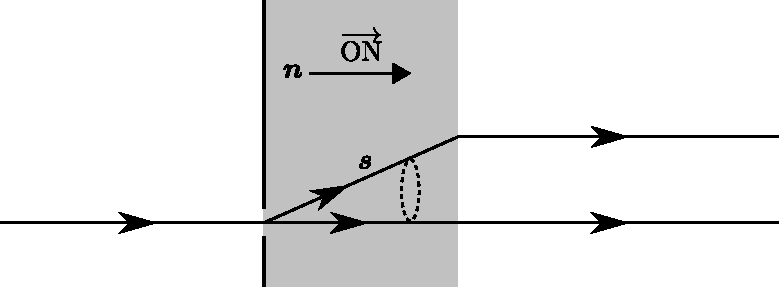
\includegraphics[scale=0.8]{innercornicalrefraction.pdf}
  \caption{双法線$(\protect\overrightarrow{\text{ON}})$向きの$\boldsymbol{n}$を持つ光は媒質に入ると内部円錐屈折を起こす}
  \label{innercornicalrefraction}
\end{figure}

外部円錐屈折を観測するには,双法線に垂直な方向に切り出した媒質を使い,それに垂直入射させる.ただし,この場合は,媒質の奥側にもスリットを置いておく.
媒質中を進むことができる光は$\boldsymbol{s}$が双径線方向の光のみである.この光の$\boldsymbol{n}$は外部円錐(図中に示した円錐)に沿って分布している.
媒質を出るときに光は屈折するが,屈折の時は群速度でなく波数が関係するのであった.2軸性媒質中と外部で,$\boldsymbol{n}$鉛直方向は変化しない.
よって,2軸性媒質を出た光はそれぞれ異なった$\boldsymbol{n}$を持つ.等方性媒質では$\boldsymbol{s}$と$\boldsymbol{n}$の向きが一致するので,媒質を出たのちの$\boldsymbol{s}$は円錐状に屈折する.
だが,$\boldsymbol{n}$の水平成分は屈折の際に変化するので,屈折後の$\boldsymbol{n}$は外部円錐に沿っていない.
そのため,$\boldsymbol{s}$も外部円錐には沿っていない.

\begin{figure}[ht]
  \centering
  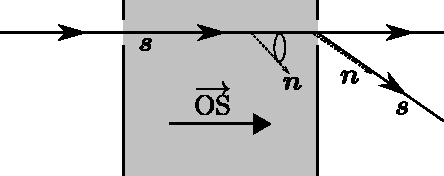
\includegraphics[scale=0.8]{outercornicalrefraction.pdf}
  \caption{外部で観測される光の向き$\boldsymbol{s}$は外部円錐と異なる}
  \label{outercornicalrefraction}
\end{figure}

円錐屈折は1832年に,W.R.Hamiltonが理論的に発見・予言し,後にH.Lloydが実験で確認した.
最近の研究で円錐屈折光からスロープ効率(定電流に対するレーザー強度)の高いレーザー発振が実現できることが分かり,レーザー結晶として使われたりする.

\relax
\section{電磁固有モード}
\paragraph{縦波モードとプラズモン}
半導体や誘電体では,価電子帯から伝導体に励起した電子と,価電子帯に残った正孔がクーロン力で結合して励起子(エキシトン)ができる.
励起子はクーロン力で結合しているので,エネルギー的に若干安定していることになる.金属でも励起子はできるが,その存在時間はとても短く観測は困難である.
最近(2017年現在)銀の励起子の寿命が長いことが分かったらしい.そのような励起子と電磁場の相互作用を考える.
まずは等方的な物質中のMaxwell方程式を記述しよう:
\begin{align}
  \dive \boldsymbol{D} &= \rho\label{long_mode_gauss}, \\
  \rot \boldsymbol{E} &= -\dfrac{\partial\boldsymbol{B}}{\partial{t}}, \\
  \rot \boldsymbol{H} &= \boldsymbol{j} + \dfrac{\partial\boldsymbol{D}}{\partial{t}}, \\
  \dive \boldsymbol{B} &= 0.
\end{align}
内部に存在する電場は
\begin{align}
  \boldsymbol{E} = \boldsymbol{E}_0\exp\left[i(\boldsymbol{k}\cdot\boldsymbol{r}-\omega{t})\right]
\end{align}
とする.これを(\ref{long_mode_gauss})に代入すると,
\begin{align}
  i\varepsilon(\omega)\boldsymbol{k}\cdot\boldsymbol{E}=\rho
\end{align}
となる.ただし,$\varepsilon(\omega)$は誘電関数である.
よって,これを解くと,
\begin{align}
  \boldsymbol{E}=\boldsymbol{E}_l=-\dfrac{i\boldsymbol{k}}{k^2\varepsilon(\omega)}\rho\label{long_mode_El}
\end{align}
となる.これは電場の波(電磁波でないことに注意)の進む方向$\boldsymbol{k}$に平行なので,縦波である.
外部電荷密度$\rho=0$の時には$E_l=0$となるが,振動子モデルで調べたように,散逸を無視した拡張振動子の誘電関数は,
\begin{align}
  \varepsilon(\omega)=\varepsilon_\text{b}+\dfrac{\varepsilon_0}{{\omega_0}^2-\omega^2}\dfrac{nq^2}{\varepsilon_0m}\label{long_mode_permittivity}
\end{align}
で与えられる.この場合は,常に$\varepsilon(\omega)=0$となる$\omega=0$が存在するので,(\ref{long_mode_El})において,$\rho=0$であっても$\boldsymbol{E}_l\neq0$となり,縦波が存在する.
以上から,縦波が存在する条件は,
\begin{align}
  \varepsilon(\omega)=0\label{long_mode_lwave}
\end{align}
である.また,この条件を満たす角振動数$\omega$は,(\ref{long_mode_permittivity})と(\ref{long_mode_lwave})から,
\begin{align}
  \omega=\omega_l=\sqrt{{\omega_0}^2+\dfrac{\varepsilon_0}{\varepsilon_\text{b}}\dfrac{nq^2}{\varepsilon_0m}}
\end{align}
となる.これを縦波の角振動数と言う.さらに,金属や電離気体では,原子核と電子間の束縛がなく,弾性定数$K=0$なので$\omega_0=0$となる.
このような物質をプラズマと言う.プラズマにおいて$\varepsilon_\text{b}=\varepsilon_0$の時の縦波の角振動数
\begin{align}
  \omega_l=\omega_p=\sqrt{\dfrac{nq^2}{\varepsilon_0m}}
\end{align}
をプラズマ角振動数と言う.

上で求めた条件(\ref{long_mode_lwave})を別の方法で導いてみよう.
物質の中に波数$\boldsymbol{k}$で表される電気分極$\boldsymbol{P}$の縦波平面波があるとする.
この時,分極電荷による反電場$\boldsymbol{E}$を考えることができるので(本当はある一点の周りの電気双極子モーメントによる電場が存在している),
\begin{align}
  \boldsymbol{E}=-\dfrac{\boldsymbol{P}}{\varepsilon_0}
\end{align}
である.さらに,$\boldsymbol{P}=\varepsilon_0\chi\boldsymbol{E}$を代入すると,$\chi=-1$となる.
これを誘電率と電気感受率の関係式$\varepsilon=\varepsilon_0(1+\chi)$に代入すると,確かに
\begin{align}
  \varepsilon=0
\end{align}
となる.プラズマの場合,縦波を発生させる復元力を担っているものは反電場なのである.
また,波の位相とほぼ等速で進む電子が電磁波の電場によってエネルギーを得るため,縦波は減衰する.これをLandau減衰と呼ぶ.
プラズマ中の自由電子は集団的に振動しているので,擬似的な粒子(量子)として振舞っていると考えることができる.これをプラズモンという.
角振動数$\omega_p$で振動するプラズモンは$\hbar\omega_p$のエネルギーを持つことのみが許される.

\paragraph{横波モードとポラリトン}
励起子と電磁場の相互作用系の縦波では,伝播する変化である電気分極$\boldsymbol{P}$に対する復元力は反電場$\boldsymbol{E}$であった.

電荷がない時のMaxwell方程式は,
\begin{align}
  \varepsilon(\omega)\boldsymbol{k}\cdot\boldsymbol{E}=0
\end{align}
となる.$\varepsilon(\omega)\neq0$の領域では,$\boldsymbol{k}\perp\boldsymbol{E}$となり,これは横波である.

拡張された電磁波動方程式\eqref{comp_wave_eq_newequationE}において散逸$\gamma$を無視したとき,波数$k$と角振動数$\omega$の分散は,
\begin{align}
  k^2=\mu_0\varepsilon_0\left(\dfrac{\varepsilon_{\text{b}}}{\varepsilon_0}+\dfrac{{\omega_p}^2}{{\omega_0}^2-\omega^2}\right)\omega^2\label{trans_mode_div}
\end{align}
で与えられる.
左辺が正なので,右辺も正でなくてはならない.よって,$\omega$が存在できる範囲は,
\begin{align}
  \omega < \omega_0 , \quad  \omega > \sqrt{{\omega_0}^2+\dfrac{\varepsilon_0}{\varepsilon_{\text{b}}}{\omega_p}^2} = \omega_l
\end{align}
となる.$\omega_l$は縦波の各振動数,$\omega_p$はプラズマ角振動数である.
(\ref{trans_mode_div})を図示すると,本文図8-19のようになる.
分散曲線が2本に分かれるのは,誘電率$\varepsilon_{\text{b}}$の物質中を進む電磁波$(\omega=c_{\text{b}}k)$と誘電体内の分極の振動$(\omega=\omega_0)$の混合状態だからである.
これをポラリトンという.

$\omega\ll\omega_0$の時は\eqref{osc_model_st}の静的な誘電率$\varepsilon_{\text{st}}$に従って速さ$c_{\text{s}}=\dfrac{c}{\sqrt{\varepsilon_{\text{st}}}}$で進む電磁波となる.

$\omega\to\omega_0-0$の時は$k,\varepsilon\to\infty$となり,これは背景媒質に関係ない分極の波になる.
なぜならば,背景媒質とは注目している分極の固有角振動数$\omega_0$よりも大きな固有角振動数を持つもののことを言うからである.
ここでは注目している分極が共鳴を起こし,背景媒質の寄与はとても小さくなる.

$\omega\to\omega_l+0$の時は$k,\varepsilon\to0$となり,これは縦波と同じ状況である.

$\omega\gg\omega_0$となると,固有角振動数$\omega_0$の分極の寄与はほとんどなくなる.その結果一定の背景媒質を進む電磁波となる.

\paragraph{プラズマの表皮効果}
プラズマに入射する電磁波のふるまいを見よう.プラズマで散逸$\gamma$が小さいとすると, 振動子モデルで考えた拡張した誘電関数において$\varepsilon_{\text{b}}=\varepsilon_0$として,
\begin{align}
  \varepsilon(\omega)=\varepsilon_0\left(\dfrac{\omega^2-{\omega_p}^2}{\omega^2}\right)
\end{align}
となる.よって,$\omega < \omega_p$のときは誘電関数が負となる.波動方程式\eqref{comp_wave_eq_newequationE}から,
\begin{align}
  n&=0\label{skin_eff_n}\\
  \kappa&=\dfrac{\sqrt{{{\omega_p}^2-\omega^2}}}{\omega}\label{skin_eff_kappa}
\end{align}
となる.$\omega_p$の値は,通常の金属では$10^{16}$程度である.これに対して可視光の$\omega$は$10^{15}\sim10^{16}$程度である.
よって,金属でほとんどの光が反射される.だが,それでも一部の光は減衰しながら金属中に侵入する.
$x$軸に伝わる電磁波を考える.$0\leq{x}$の適当な範囲にプラズマが存在するとしよう(本文図8-9みたいな感じ).

(\ref{skin_eff_n})と(\ref{skin_eff_kappa})を減衰を考えた電場\eqref{comp_wave_eq_E}に代入して,
\begin{align}
  \boldsymbol{E}=\boldsymbol{E}_0\exp\left(-\dfrac{\sqrt{{{\omega_p}^2-\omega^2}}}{c}x\right)\exp(-i\omega{t})
\end{align}
を得る.これは,$x$軸方向に減衰する波を表す.この式からも分かるように,波は薄いプラズマ中では完全に0になる訳ではない.このようなものを消衰波と言う.
静電場がかかっていればプラズマ中では静電誘導により電場が0となるが,これは時間的に変動する電場なので静電誘導は起こらない.電磁波の場合は消衰波ができ,電場が弱くなる.
これを表被効果という.

\paragraph{ヘリコン波とホイスラー波}
プラズマ角振動数$\omega_p$より角振動数$\omega$が小さい電磁波はプラズマ中では伝播できないことが分かった.
だが,特別な場合はそのような電磁波であっても伝播できる.

\eqref{e_diople_in_m_tensor}から,$\zeta$方向に磁場がかかっている時の感受率テンソルは,
\begin{align}
  \chi =
  \dfrac{{\omega_p}^2}{\omega}\left(
  \begin{array}{ccc}
    \dfrac{\omega+i\gamma}{{\omega_c}^2-(\omega+i\gamma)^2} & \dfrac{i\omega_c}{{\omega_c}^2-(\omega+i\gamma)^2} & 0 \\ \\
    \dfrac{-i\omega_c}{{\omega_c}^2-(\omega+i\gamma)^2} & \dfrac{\omega+i\gamma}{{\omega_c}^2-(\omega+i\gamma)^2} & 0 \\ \\
    0 & 0 & \dfrac{-1}{\omega+i\gamma}
  \end{array}
  \right)
\end{align}
である.プラズマなので$\omega_0=0$である.散逸$\gamma$を無視すれば,
\begin{align}
  \chi =
  \dfrac{{\omega_p}^2}{\omega}\left(
  \begin{array}{ccc}
    \dfrac{\omega}{{\omega_c}^2-\omega^2} & \dfrac{i\omega_c}{{\omega_c}^2-\omega^2} & 0 \\ \\
    \dfrac{-i\omega_c}{{\omega_c}^2-\omega^2} & \dfrac{\omega}{{\omega_c}^2-\omega^2} & 0 \\ \\
    0 & 0 & -\dfrac{1}{\omega}
  \end{array}
  \right)
  \label{helicon_tensor}
\end{align}
$\zeta$正の向きに進む円偏光の電場は,
\begin{align}
  E_{\xi} &= iE_{\eta} , \quad  E_{\zeta}=0 ~ (\text{Right}) \label{helicon_right}\\
  E_{\eta} &= iE_{\xi} , \quad E_{\zeta}=0 ~ (\text{Left}) \label{helicon_left}
\end{align}
である.背景媒質$\varepsilon_{\text{b}}$でのポラリトンに対する拡張誘電関数は
\begin{align}
  \boldsymbol{D} &= \varepsilon_{\text{b}}\boldsymbol{E}+\boldsymbol{P}\notag\\
  &= \varepsilon_{\text{b}}\boldsymbol{E}+\varepsilon_0\chi\boldsymbol{E}\notag\\
  &= \varepsilon\boldsymbol{E}
\end{align}
このように決定される.ここで,一般に$\chi$と$\varepsilon$は2階のテンソルであるが,これを0階のテンソルに直すことを考える.右周りの円偏光に対しては,
\begin{align}\left(
  \begin{array}{c}
    D_{\xi} \\
    D_{\eta} \\
    D_{\zeta}
  \end{array}
  \right)
  &=
  \varepsilon_{\text{b}}
  \left(
  \begin{array}{c}
    iE_{\eta} \\
    E_{\eta} \\
    0
  \end{array}
  \right)
  +
  \dfrac{\varepsilon_0{\omega_p}^2}{\omega}\left(
  \begin{array}{ccc}
    \dfrac{\omega}{{\omega_c}^2-\omega^2} & \dfrac{i\omega_c}{{\omega_c}^2-\omega^2} & 0 \\ \\
    \dfrac{-i\omega_c}{{\omega_c}^2-\omega^2} & \dfrac{\omega}{{\omega_c}^2-\omega^2} & 0 \\ \\
    0 & 0 & -\dfrac{1}{\omega}
  \end{array}
  \right)
  \left(
  \begin{array}{c}
    iE_{\eta} \\
    E_{\eta} \\
    0
  \end{array}
  \right)\notag\\
  &=
  \left[\varepsilon_{\text{b}}+\dfrac{\varepsilon_0{\omega_p}^2}{\omega(\omega_c-\omega)}\right]
  \left(
  \begin{array}{c}
    iE_{\eta} \\
    E_{\eta} \\
    0
  \end{array}
  \right)
\end{align}
よって,右回りの円偏光に対する誘電率は
\begin{align}
  \varepsilon_{\text{R}}=\varepsilon_{\text{b}}+\dfrac{\varepsilon_0{\omega_p}^2}{\omega(\omega_c-\omega)}\label{helicon_perR}
\end{align}
で与えられる.同様に,左回りの円偏光に対する誘電率は
\begin{align}
  \varepsilon_{\text{L}}=\varepsilon_{\text{b}}-\dfrac{\varepsilon_0{\omega_p}^2}{\omega(\omega_c+\omega)}\label{helicon_perL}
\end{align}
で与えられる.$\omega_c=\dfrac{qB}{m}$はプラズマの荷電粒子と同じ符号を持つ.
よって,荷電粒子が正孔などの場合は$\varepsilon_{\text{R}}$,自由電子などの場合は$\varepsilon_{\text{L}}$が極を持つ.
$|\omega_c|$と$\omega$が一致するということは,サイクロトロン運動する荷電粒子と電磁波が共鳴するということである.これをサイクロトロン共鳴と言う.
ところで,(\ref{helicon_perR})と(\ref{helicon_perL})において$\omega$が十分小さいときは,
\begin{align}
  \varepsilon_{\text{R}} &= \dfrac{\varepsilon_0{\omega_p}^2}{\omega\omega_c}\label{helicon_perHR}\\
  \varepsilon_{\text{L}} &= -\dfrac{\varepsilon_0{\omega_p}^2}{\omega\omega_c}\label{helicon_perHL}
\end{align}
と近似される.荷電粒子が正孔などの場合は$\varepsilon_{\text{R}} > 0$となり右回りの偏光のみが伝播する.
一方で自由電子などの場合は$\varepsilon_{\text{L}} > 0$となり左回りの偏光のみが伝播する.

表皮効果で調べたように,プラズマ角振動数$\omega_p$より角振動数$\omega$が小さい電磁波はプラズマの中では減衰してしまう.
だが,磁場が存在するとプラズマ振動数よりも低い振動数の電磁波も伝わることができる.この波は電磁波とサイクロトロン運動の混成波で,ヘリコン波と言う.
ヘリコン波の分散は,ヘリコン波の角振動数を$\omega_\text{H}$とすると,
\begin{align}
  \varepsilon\mu_0=\dfrac{k^2}{{\omega_\text{H}}^2}
\end{align}
に(\ref{helicon_perHR}),(\ref{helicon_perHL})を代入して,
\begin{align}
  \omega_{\text{H}}=\dfrac{|\omega_c|}{\varepsilon_0\mu_0{\omega_p}^2}k^2=\dfrac{H}{n|q|}k^2
\end{align}
で与えられる.ただし,$H$は磁場の大きさである.

これと同じことが地球表面で起きており,電離層中を地磁気に沿って伝搬する電磁波をホイスラー波と呼ぶ.
南半球で発生した雷の信号が地磁気の磁力線に沿ってホイッスル状の雑音として北半球まで伝わることからこの名前がついている.

\paragraph{表面ポラリトン}
散逸を$\gamma$を無視した横波において,その分散は,
\begin{align}
  k^2=\mu_0\varepsilon_0\left(\dfrac{\varepsilon_{\text{b}}}{\varepsilon_0}+\dfrac{{\omega_p}^2}{{\omega_0}^2-\omega^2}\right)\omega^2
  \label{surface_traDiv}
\end{align}
で表される.これが横波として減衰せずに存在するためには,両辺正であることが必要である.
複素電磁方程式で導入した複素波数ベクトル\eqref{comp_wave_eq_Ek}において,虚部が正であれば減衰が起こるのであった.
よって,(\ref{surface_traDiv})において比誘電率$\tilde{\varepsilon}$が,
\begin{align}
  \tilde{\varepsilon}=\dfrac{\varepsilon_{\text{b}}}{\varepsilon_0}+\dfrac{{\omega_p}^2}{{\omega_0}^2-\omega^2} < 0
\end{align}
であれば横波はすぐに消衰し,表面のみに存在できることが分かる.

\begin{figure}[ht]
  \centering
  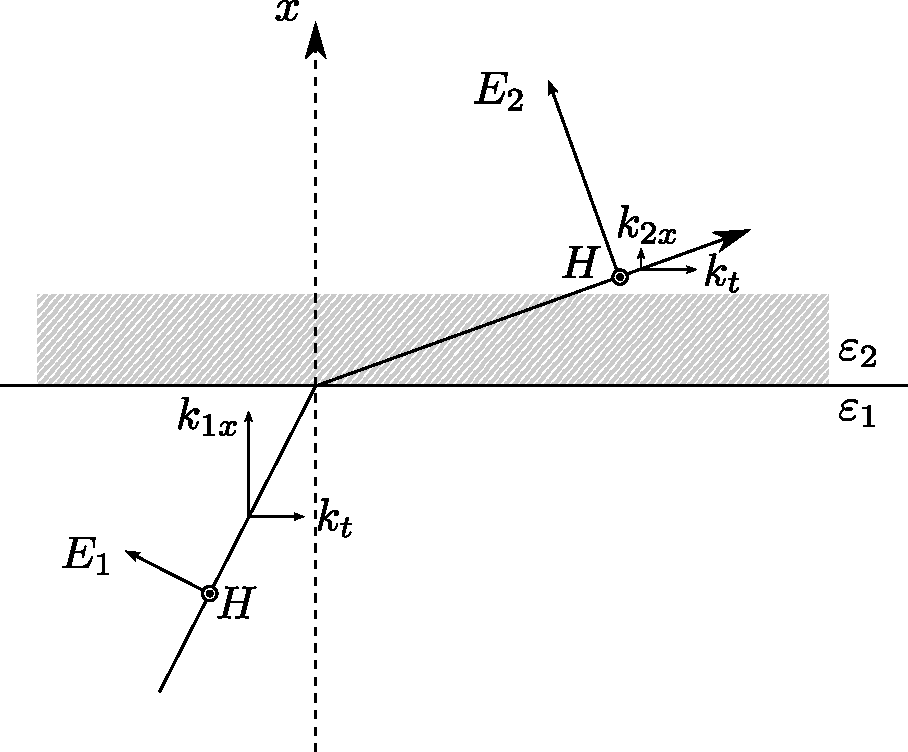
\includegraphics[scale=0.5]{TMrec.pdf}
  \caption{電磁波はTM波(磁場が入射面に平行な波;p偏光)とする}
  \label{TMrec}
\end{figure}

ここで,図のように誘電率$\varepsilon_1$の物質から誘電率$\varepsilon_2$の物質に入射する電磁波を考える.
電磁波の屈折や透過,反射において反射面に平行な波数は変化しないので,それを$k_t$とおいた.
両方の物質内で,電荷が存在しないとすると$\dive\boldsymbol{D}=0$なので,
\begin{align}
  k_tE_{1t}+k_{1x}E_{1x}=0\label{surface_E1} \\
  k_tE_{2t}+k_{2x}E_{2x}=0\label{surface_E2}
\end{align}
となる.さらに,境界において,電場の面に接する向きの成分は連続であり,電束密度の法線方向は連続であるので,
\begin{align}
  E_{1t}&=E_{2t}=E_t\label{surface_E} \\
  \varepsilon_1E_{1x}&=\varepsilon_2E_{2x}\label{surface_D}
\end{align}
となる.(\ref{surface_E1}),(\ref{surface_E2}),(\ref{surface_E}),(\ref{surface_D})から,
\begin{align}
  \varepsilon_2k_{1x}=\varepsilon_1k_{2x}\label{surface_epsK}
\end{align}
となる.両物質で透磁率がともに$\mu_0$であるとすると,電磁波の屈折や透過,反射において$\omega$は変化しないことから,
\begin{align*}
  \dfrac{\omega^2}{{k_{1t}}^2+{k_{1x}}^2}=\dfrac{\omega^2}{{k_1}^2}={c_1}^2=\dfrac{1}{\mu_0\varepsilon_1}=\dfrac{1}{\mu_0\varepsilon_0}\dfrac{\varepsilon_0}{\varepsilon_1}
  =c^2\dfrac{\varepsilon_0}{\varepsilon_1}=\dfrac{\omega^2}{{k}^2}\dfrac{\varepsilon_0}{\varepsilon_1}
\end{align*}
などの計算をして,
\begin{align}
  {k_{1t}}^2+{k_{1x}}^2=\dfrac{\varepsilon_1}{\varepsilon_0}k^2\label{surface_k1} \\
  {k_{2t}}^2+{k_{2x}}^2=\dfrac{\varepsilon_2}{\varepsilon_0}k^2\label{surface_k2}
\end{align}
となる.ただし,$k$は真空中での波数である.(\ref{surface_epsK}),(\ref{surface_k1}),(\ref{surface_k2})から,
\begin{align}
  {k_{1x}}^2&=\dfrac{{\varepsilon_1}^2}{\varepsilon_0(\varepsilon_1+\varepsilon_2)}k^2\label{surface_k1x}\\
  {k_{2x}}^2&=\dfrac{{\varepsilon_2}^2}{\varepsilon_0(\varepsilon_1+\varepsilon_2)}k^2\label{surface_k2x}\\
  {k_{t}}^2&=\dfrac{\varepsilon_1\varepsilon_2}{\varepsilon_0(\varepsilon_1+\varepsilon_2)}k^2\label{surface_kt}\\
\end{align}
となる.ここで,$k_t$が実数の下で$\varepsilon_1$の物質と$\varepsilon_2$の物質の中で電磁波が共に消衰波となるのは,
\begin{align}
  {k_{1x}}^2 < 0 \quad \text{かつ} \quad {k_{2x}}^2 < 0
\end{align}
の時である.(\ref{surface_k1x}),(\ref{surface_k2x})から,これは
\begin{align}
  \varepsilon_1\varepsilon_2 < 0 \quad \text{かつ} \quad \varepsilon_1+\varepsilon_2 < 0\label{surface_epsCond}
\end{align}
に対応する.この時,波は両側で消衰波となり,表面にのみ局在できる.

$\varepsilon_2$を拡張振動子モデルで散逸を無視したものとすると,
$\varepsilon_1$が真空で,$\varepsilon_2$の散逸$\gamma$が十分小さいときは,(\ref{surface_kt})から,
\begin{align}
  k_t=\dfrac{\omega}{c}\sqrt{\left(\dfrac{\varepsilon_{\text{b}}}{\varepsilon_0}+\dfrac{{\omega_p}^2}{{\omega_0}^2-\omega^2}\right)
  \left(1+\dfrac{\varepsilon_{\text{b}}}{\varepsilon_0}+\dfrac{{\omega_p}^2}{{\omega_0}^2-\omega^2}\right)^{-1}}
\end{align}
となる.ただし,(\ref{surface_epsCond})から,
\begin{align}
  \tilde{\varepsilon}_2=\dfrac{\varepsilon_{\text{b}}}{\varepsilon_0}+\dfrac{{\omega_p}^2}{{\omega_0}^2-\omega^2} < -1
\end{align}
である.これを変形すると,$\omega$の存在範囲は,
\begin{align}
  \omega_0+0 < \omega < \sqrt{{\omega_0}^2+\dfrac{\varepsilon_0}{\varepsilon_0+\varepsilon_{\text {b}}}{\omega_p}^2}=\omega_s
\end{align}
となる.この$\omega_s$を表面プラズマ角振動数と呼ぶ.
以上から,表面波の分散は,本文図8-21のようになる.

このような表面波を表面波ポラリトンと呼ぶ.これは,分極電荷の振動と電磁波の混成である.
表面波ポラリトンは,波数$k_t$で表面に沿って伝播する.
誘電体表面には,面密度$\sigma_P=P_n(\boldsymbol{r})$の分極電荷が分布していると考えることができるのであった.
よって,分極電荷の振幅は,
\begin{align}
  \sigma_P&=-P_{2x}\notag\\
  &=-D_{2x}-\varepsilon_0E_{2x}\notag\\
  &=-(\varepsilon_2-\varepsilon_0)E_{2x}\notag\\
  &=-i(\varepsilon_2-\varepsilon_0)\dfrac{k_t}{|k_{2x}|}E_t
\end{align}
となる.$x$軸の向きは誘電体の内側に向かっている.
$\varepsilon_2 < 0$より,$E_t$の位相は$\sigma_P$の位相より$\dfrac{\pi}{2}$遅れていることが分かる.


\end{document}
